\documentclass[11pt,a4paper,twoside]{article}

% Paquetes (añade otros si los necesitas):

\usepackage[T1]{fontenc}
\usepackage[utf8]{inputenc}
\usepackage{float}

% Style package
% Font Package (Palatino)
\usepackage{mathpazo}
% Packages for specific capabilities
\usepackage{rotating} % for text rotation in tables
\usepackage{multirow} % for multirow in tables
\usepackage{subfigure} % Place subfigures in figure environment
% Packages for specific symbols
\usepackage{amssymb}
\usepackage{amsmath}
\usepackage{amsfonts}
\usepackage{eurosym} % Euro symbol
\usepackage{bbding} % for \XSolidBrush
\usepackage{pifont} % for \ding{55} (a check mark)


\usepackage{latexsym}
\usepackage{tikz}
\usetikzlibrary{arrows.meta,babel,positioning,shapes.geometric,calc}
\usepackage{soul}
\usepackage{array}
%\usepackage{marvosym}
\usepackage{epsfig}
\usepackage{graphics}
\usepackage{amsfonts}
\usepackage{xspace}
\usepackage{color}
\usepackage{booktabs}
% \usepackage{parskip} % Comentado para habilitar la sangría (indentación) en los párrafos
\usepackage{xtab}
\usepackage[numbers,sort&compress]{natbib}
\usepackage[colorlinks=true,urlcolor=blue,linkcolor=blue,citecolor=blue]{hyperref}
\numberwithin{equation}{section}




\linespread{1.05}

% TFG en inglés:
%\usepackage[english]{babel} 
%\addto\captionsenglish{\renewcommand{\chaptername}{}}

% TFG en español:
\usepackage[spanish,es-nodecimaldot,es-tabla,es-lcroman,es-nosectiondot]{babel}
\renewcommand\spanishchaptername{}

% Formato de la página:
\usepackage{fancyhdr}
\usepackage[top=2.88cm,bottom=2.97cm,left=2.95cm,right=2.95cm]{geometry}
\setlength{\parskip}{0.1cm}
\setlength{\parindent}{1.5em} % Añadida sangría para la primera línea de cada párrafo
\raggedbottom
% Pon aquí tus definiciones:

\newcommand{\dis}{\displaystyle}
%\sodef\an{}{.2em}{1em plus1em}{2em plus.1em minus.1em}

\begin{document}

% Portada %%%%%%%%%%%%%%%%%%%%%%%%%%%%%%%%%%%%%%%%%%%%%%%%%%%%%%%%%%%%%%%%%%%%%%

\pagestyle{empty}


\noindent
\begin{tabular}{r}

\includegraphics[width=8.8cm]{img/escudoUGRmonocromo.png} \\[-1.8ex]
\hspace{31mm}\vspace{-8mm}
\begin{tabular}{c}
\hline\\[-1ex]\hskip-2mm
{\bf Facultad de Ciencias}\hspace{18mm}
\end{tabular}
\end{tabular}

\large
\vspace{30mm}
\hspace{25mm}
\begin{tabular}{l}
GRADO EN F\'ISICA
\end{tabular}

\vspace{45mm}
\hspace{25mm}
\begin{tabular}{p{13cm}}
TRABAJO FIN DE GRADO
\\[1.5ex]
\LARGE\bf Análisis del efecto de la difracción en la estimación del campo magnético solar mediante la aproximación de campo débil (WFA) a partir de datos del instrumento TuMag a bordo de Sunrise III
\end{tabular}
%
\vfill
\hspace{25mm}
\begin{tabular}{l}
Presentado por:
\\
{\bf D. Pablo Orellana Chornyak}
\\[3ex]
Curso Académico 2025/2026
\end{tabular}
%

\newpage
%
\begin{center}
{\bf Resumen}
\bigskip

\begin{minipage}{0.8\linewidth}
Este estudio aborda la mitigación de la degradación óptica (difracción y aberraciones) en observaciones espectropolarimétricas solares de alta resolución del instrumento TuMag (misión Sunrise III). El objetivo es inferir el campo magnético longitudinal del ``Sol en calma'' mediante la Aproximación de Campo Débil (WFA). Dado que las técnicas clásicas de deconvolución de imágenes presentan dificultades al aplicarse sobre la componente $V$ de Stokes ---por su naturaleza bipolar y la no linealidad del problema---, se ha implementado una metodología de modelado directo espacialmente acoplado. Basado en el marco de van Noort, este método integra la óptica del telescopio y la física de transferencia radiativa. Al resolver el sistema iterativamente con el método del Gradiente Conjugado, sin guardar la matriz Jacobiana en memoria, se consigue reconcentrar el flujo magnético. Las pruebas sobre datos sintéticos muestran una recuperación de la señal frente al ruido instrumental, mientras que su aplicación en observaciones reales indica una mejora de la topología magnética acorde a lo esperado.
\end{minipage}

\vfill

{\bf Abstract} 
\bigskip

\begin{minipage}{0.8\linewidth}
This study addresses the mitigation of optical degradation (diffraction and aberrations) in high-resolution solar spectropolarimetric observations from the TuMag instrument (Sunrise III mission). The objective is to infer the longitudinal magnetic field of the ``quiet Sun'' using the Weak Field Approximation (WFA). Given that classical image deconvolution techniques face difficulties when applied to the Stokes $V$ component ---due to its bipolar nature and the non-linearity of the problem---, a spatially coupled forward modeling methodology has been implemented. Based on van Noort's framework, this method integrates the telescope's optics and radiative transfer physics. By solving the system iteratively via the Conjugate Gradient method without instantiating the Jacobian matrix, a coherent reconcentration of the scattered magnetic flux is achieved. Tests on synthetic data show the signal retrieval in the presence of instrumental noise, while its application to real observations suggests a reconcentration of the magnetic topology consistent with expectations.
\end{minipage}

\vfill

\end{center}

\newpage

% Indice %%%%%%%%%%%%%%%%%%%%%%%%%%%%%%%%%%%%%%%%%%%%%%%%%%%%%%%%%%%%%%%%%%%%%%%
%\newpage
\begingroup
\setlength{\parskip}{0pt}
\tableofcontents
\endgroup
% Texto %%%%%%%%%%%%%%%%%%%%%%%%%%%%%%%%%%%%%%%%%%%%%%%%%%%%%%%%%%%%%%%%%%%%%%%%
%\newpage

\pagestyle{fancy}
\fancyhead[RO,LE]{\leftmark}
\fancyhead[LO,RE]{\thepage}
\fancyfoot{}

\newpage

% !TeX root = ../main.tex

\section{Introducción y motivación}
Uno de los ámbitos más importantes en la astrofísica actual es el estudio de nuestro propio Sol. Los múltiples fenómenos físicos que presenta nos ayudan a comprender el comportamiento de otras estrellas, convirtiéndolo en un área de investigación muy activa. Para profundizar en su estudio, se han desarrollado observatorios como Sunrise \cite{Barthol2011}, un telescopio montado en un globo estratosférico que permite esquivar gran parte de la atmósfera terrestre. Gracias a instrumentos a bordo como TuMag \cite{SUNRISETuMagTUMAGData}, es posible obtener imágenes magnéticas solares de alta calidad y resolución espacial.

Sin embargo, el problema a resolver radica en que, a pesar de operar por encima de la atmósfera, el propio instrumento sufre los efectos de la difracción de la luz y de aberraciones ópticas. Para lograr imágenes nítidas de regiones muy pequeñas del Sol, es necesario contrarrestar estos defectos. A este proceso computacional que corrige la degradación espacial de las imágenes se le llama deconvolución.

Un aspecto fundamental del estudio solar es su campo magnético. Aunque una parte de este magnetismo se manifiesta en procesos a gran escala y muy energéticos, como las manchas solares, una fracción nada despreciable se encuentra en lo que se conoce como el ``Sol en calma'' \cite{BellotRubio2019}. En esta región destacan los gránulos solares, células convectivas de plasma situadas en la fotosfera. Estas estructuras presentan un campo magnético débil (del orden de cientos de Gauss) y son un gran foco de investigación, ya que aún se debate si su magnetismo es generado por el propio movimiento del plasma a nivel local, o si es un reflejo del campo magnético interno que emerge a la superficie.

Describir teóricamente la interacción entre el campo magnético y la luz es un reto complejo. En la literatura se han desarrollado modelos que, a través de los parámetros de Stokes, nos permiten medir estos campos magnéticos. Una de estas aproximaciones teóricas, y el pilar fundamental de este proyecto, es la aproximación de campo débil \cite{cteGeff}. Utilizando desarrollos de Taylor de primer orden, esta aproximación nos permite deducir el campo magnético de forma directa a partir de los perfiles de Stokes, facilitando el estudio del Sol en calma y de los gránulos solares.

Precisamente, afrontar el reto computacional y físico de deconvolucionar estas imágenes integrando la información del campo magnético ha sido el objetivo principal de este proyecto. Poder trabajar con datos de misiones aeroespaciales, conocer la investigación actual de primera mano, aprender de los investigadores del Departamento de Física Solar del Instituto de Astrofísica de Andalucía (IAA) y contribuir con un nuevo algoritmo han sido las principales motivaciones de este trabajo.

Para lograr este objetivo, el presente documento se estructura de la siguiente manera: en primer lugar, se explican los fundamentos teóricos sobre datos espectrales y transferencia radiativa, necesarios para derivar la expresión del campo magnético objeto de estudio. A continuación, se describe el problema de la degradación espacial de las imágenes y los retos asociados a la recolección de datos con telescopios, introduciendo así el concepto de deconvolución. Después, se presenta el estado actual de las técnicas de deconvolución más clásicas aplicadas a imágenes convencionales. Tras ello, se propone y desarrolla un nuevo método para restaurar los mapas de campo magnético basándose en la literatura científica reciente. Posteriormente, se analizan tanto los algoritmos tradicionales (implementados como parte de este trabajo) como el nuevo método propuesto, evaluando sus resultados en datos sintéticos mediante diversas métricas. Por último, se aplica el método desarrollado a datos observacionales reales recogidos por el instrumento TuMag, evaluando cualitativamente los resultados obtenidos. Además, las tecnologías y herramientas computacionales empleadas en el desarrollo de este trabajo se detallan en el Apéndice \ref{sec:tecnologias_usadas}.

\subsection{Aportación personal del trabajo}
Para aclarar el alcance de este trabajo, es importante distinguir entre los conceptos extraídos de la literatura y el trabajo desarrollado de forma autónoma. Toda la fundamentación teórica (tanto física como matemática) procede de la bibliografía citada. Por su parte, la aportación personal de este proyecto se centra en los siguientes puntos:

\begin{itemize}
    \item \textbf{Programación de todos los algoritmos:} Aunque los métodos clásicos de deconvolución no se han desarrollado teóricamente, se han programado desde cero todos los algoritmos involucrados en este trabajo, evitando el uso de ``cajas negras'' preexistentes.
    \item \textbf{Aplicación del método de van Noort:} Se ha adaptado e implementado de manera teórica el modelo directo derivado del método de van Noort (descrito en la segunda mitad de la Sección 5), aplicándolo específicamente a la recuperación del campo magnético.
    \item \textbf{Diseño de pruebas sintéticas y análisis de resultados:} Se han concebido y diseñado todos los experimentos sobre datos sintéticos para validar el correcto funcionamiento de los métodos desarrollados, simulando su respuesta frente a ópticas reales y ruido. Posteriormente, se han aplicado métricas de evaluación para analizar exhaustivamente los resultados computacionales obtenidos.
    \item \textbf{Aplicación a datos reales:} Finalmente, se ha aplicado la solución desarrollada a datos empíricos provenientes del instrumento TuMag, interpretando los resultados y redactando las conclusiones del trabajo.
\end{itemize}
% !TeX root = ../main.tex

\section{Fundamentos Teóricos}
\subsection{Datos espectrales, parámetros de Stokes}
Primero, para situarnos dentro del tema, vamos a definir exactamente qué estamos midiendo. Toda la información que extraemos del Sol proviene de las propiedades de la luz, o lo que es lo mismo, de las ondas electromagnéticas. Cuando medimos el Sol, el rango de longitudes de onda que se usará en este proyecto entra en el de la luz visible (entre $4000 - 7000$ \AA). La principal limitación de trabajar con luz visible radica en que medir directamente las propiedades de su campo electromagnético (como la amplitud o la fase) es tecnológicamente inviable debido a sus altísimas frecuencias. \\

Por lo tanto, los telescopios no miden el campo eléctrico directamente, sino que su respuesta es proporcional a la energía electromagnética promediada en el tiempo (la intensidad). Para poder medir el flujo de la energía además de las propiedades electromagnéticas, se usa el tensor de polarización. 

Para entender el tensor primero hay que entender cómo se entiende matemáticamente la polarización de una onda electromagnética. Podemos entender una onda polarizada como suma de dos ondas una en cada eje de coordenadas, los dos transversales a la dirección de propagación, con la misma frecuencia pero distinto desfase. En la siguiente figura (\ref{fig:componentes_em}) se muestra cómo la onda final es la suma de distintas ondas.

\begin{figure}[H]
    \centering
    \begin{tikzpicture}[
        >=Stealth, % Tipo de flecha elegante y matemática
        thick,
        scale=1.2 % Permite escalar el gráfico fácilmente
    ]

        % --- CONFIGURACIÓN DE COLORES ---
        % Colores elegantes basados en tu boceto
        \definecolor{vectorblue}{RGB}{41, 121, 255}
        \definecolor{compgreen}{RGB}{46, 125, 50}
        \definecolor{axesgray}{RGB}{100, 110, 120}

        % --- EJES DE COORDENADAS ---
        % Dibujamos las líneas de los ejes cruzando el origen
        \draw[->, color=axesgray, line width=0.8pt] (-3,0) -- (3,0);
        \draw[->, color=axesgray, line width=0.8pt] (0,-3) -- (0,3);

        % --- CÍRCULO DE REFERENCIA ---
        % Círculo con una línea fina y gris para no restar protagonismo
        \draw[color=axesgray!40, line width=0.8pt] (0,0) circle (2.2cm);

        % --- PARÁMETROS DEL VECTOR ---
        % Definimos el ángulo (ej. 43 grados) y el radio (2.2 cm)
        \def\angulo{43}
        \def\radio{2.2}

        % Calculamos los puntos clave automáticamente usando coordenadas polares
        \coordinate (Origen) at (0,0);
        \coordinate (E) at (\angulo:\radio); % Extremo del vector azul
        \coordinate (Ex) at ({\radio*cos(\angulo)}, 0); % Extremo componente X
        \coordinate (Ey) at (0, {\radio*sin(\angulo)}); % Extremo componente Y

        % --- LÍNEAS DE PROYECCIÓN ---
        % Líneas discontinuas desde la punta del vector a los ejes
        \draw[dashed, color=compgreen, line width=0.7pt] (E) -- (Ex);
        \draw[dashed, color=compgreen, line width=0.7pt] (E) -- (Ey);

        % --- VECTORES COMPONENTES (VERDES) ---
        \draw[->, color=compgreen, line width=1.5pt] (Origen) -- (Ex) 
            node[below, yshift=-2pt] {$E_x$};
        \draw[->, color=compgreen, line width=1.5pt] (Origen) -- (Ey) 
            node[below right, xshift=2pt, yshift=-2pt] {$E_y$};

        % --- VECTOR RESULTANTE (AZUL) ---
        \draw[->, color=vectorblue, line width=1.8pt] (Origen) -- (E);

    \end{tikzpicture}
    \caption{Componente de una onda electromagnética polarizada como suma de dos ondas en los ejes $x$ y $y$, con la misma frecuencia pero distinto desfase.}
    \label{fig:componentes_em}
\end{figure}

Por lo tanto, el tensor que usamos para medir tanto la intensidad como el desfase de la onda tiene la forma (\ref{eq: tensorDePolarizacion}), donde $\langle \cdot \rangle$ denota el promedio en el tiempo. \cite[cap. 2.3]{toroiniestaIntroductionSpectropolarimetry2003}

\begin{equation}
    \label{eq: tensorDePolarizacion}
    C \equiv \begin{pmatrix} \langle E_x E_x^* \rangle & \langle E_x E_y^* \rangle \\ \langle E_y E_x^* \rangle & \langle E_y E_y^* \rangle \end{pmatrix}
\end{equation}

Esta matriz usa números complejos, números que tienen el problema de que no son medibles realmente. Por lo tanto se utiliza una combinación lineal de los elementos de la matriz llamados parámetros de Stokes. Estos son números reales con unidades de energía, por lo que realmente podemos usarlos como medidas del telescopio. Las expresiones de los parámetros de Stokes se muestran en las expresiones (\ref{eq:stokes}). \cite[cap. 2.4]{toroiniestaIntroductionSpectropolarimetry2003}
\begin{equation}
    \label{eq:stokes}
    \begin{aligned}
        I &\equiv \kappa (C_{11} + C_{22}) \\
        Q &\equiv \kappa (C_{11} - C_{22}) \\
        U &\equiv \kappa (C_{12} + C_{21}) \\
        V &\equiv i\kappa (C_{21} - C_{12})
    \end{aligned}
\end{equation}

Donde $\kappa$ es un factor de proporcionalidad que depende de la luz y del telescopio. 

Desde un punto de vista físico, cada uno de los parámetros de Stokes tiene un significado.

\begin{itemize}
    \item $I$ es la intensidad total de la luz, es decir, la energía electromagnética que llega al detector por unidad de tiempo y superficie. Representa el brillo global de la señal.
    \item $Q$ mide la diferencia entre la polarización lineal horizontal y la vertical, es decir, entre 0\,deg y 90\,deg.
    \item $U$ mide la diferencia entre dos orientaciones diagonales de la polarización lineal, a 45\,deg y 135\,deg.
    \item $V$ cuantifica la polarización circular y permite distinguir si domina la componente derecha o la izquierda.
\end{itemize}

Donde medir $V$ es especialmente importante, ya que nos permitirá poder medir el campo magnético del Sol, como explicaremos más adelante.



\subsubsection{Qué significa la gaussiana}

\subsection{Campo magnético y aproximación de campo débil}

\begin{equation}
    \label{eq:campoDebil}
    V = -C g_{eff} \lambda^2 B_{\parallel} \frac{d I_0}{d \lambda}
\end{equation}

% !TeX root = ../main.tex

\section{Degradación espacial de imágenes: PSF, emborronamiento y deconvolución}

Un telescopio real afecta a una imagen mediante una operación llamada convolución. En esta operación, la imagen que se obtiene es el resultado de la convolución de la imagen real con una función que se llama función de punto extendido, PSF (\textit{Point Spread Function}). La PSF describe cómo un punto de luz se extiende en la imagen debido a los efectos de desenfoque, aberraciones, difracción, etc. 

Matemáticamente se describe de esta manera:

\begin{equation}
    \label{eq:convolucion}
    d_{observado} = d_{real} * p
\end{equation}


En esta expresión, $d_{observado}$ es la imagen adquirida por el telescopio, $d_{real}$ es el objeto extenso original, y $p$ es la PSF del sistema óptico. A modo ilustrativo, se presenta la siguiente figura:


\begin{figure}[H]
    \centering
    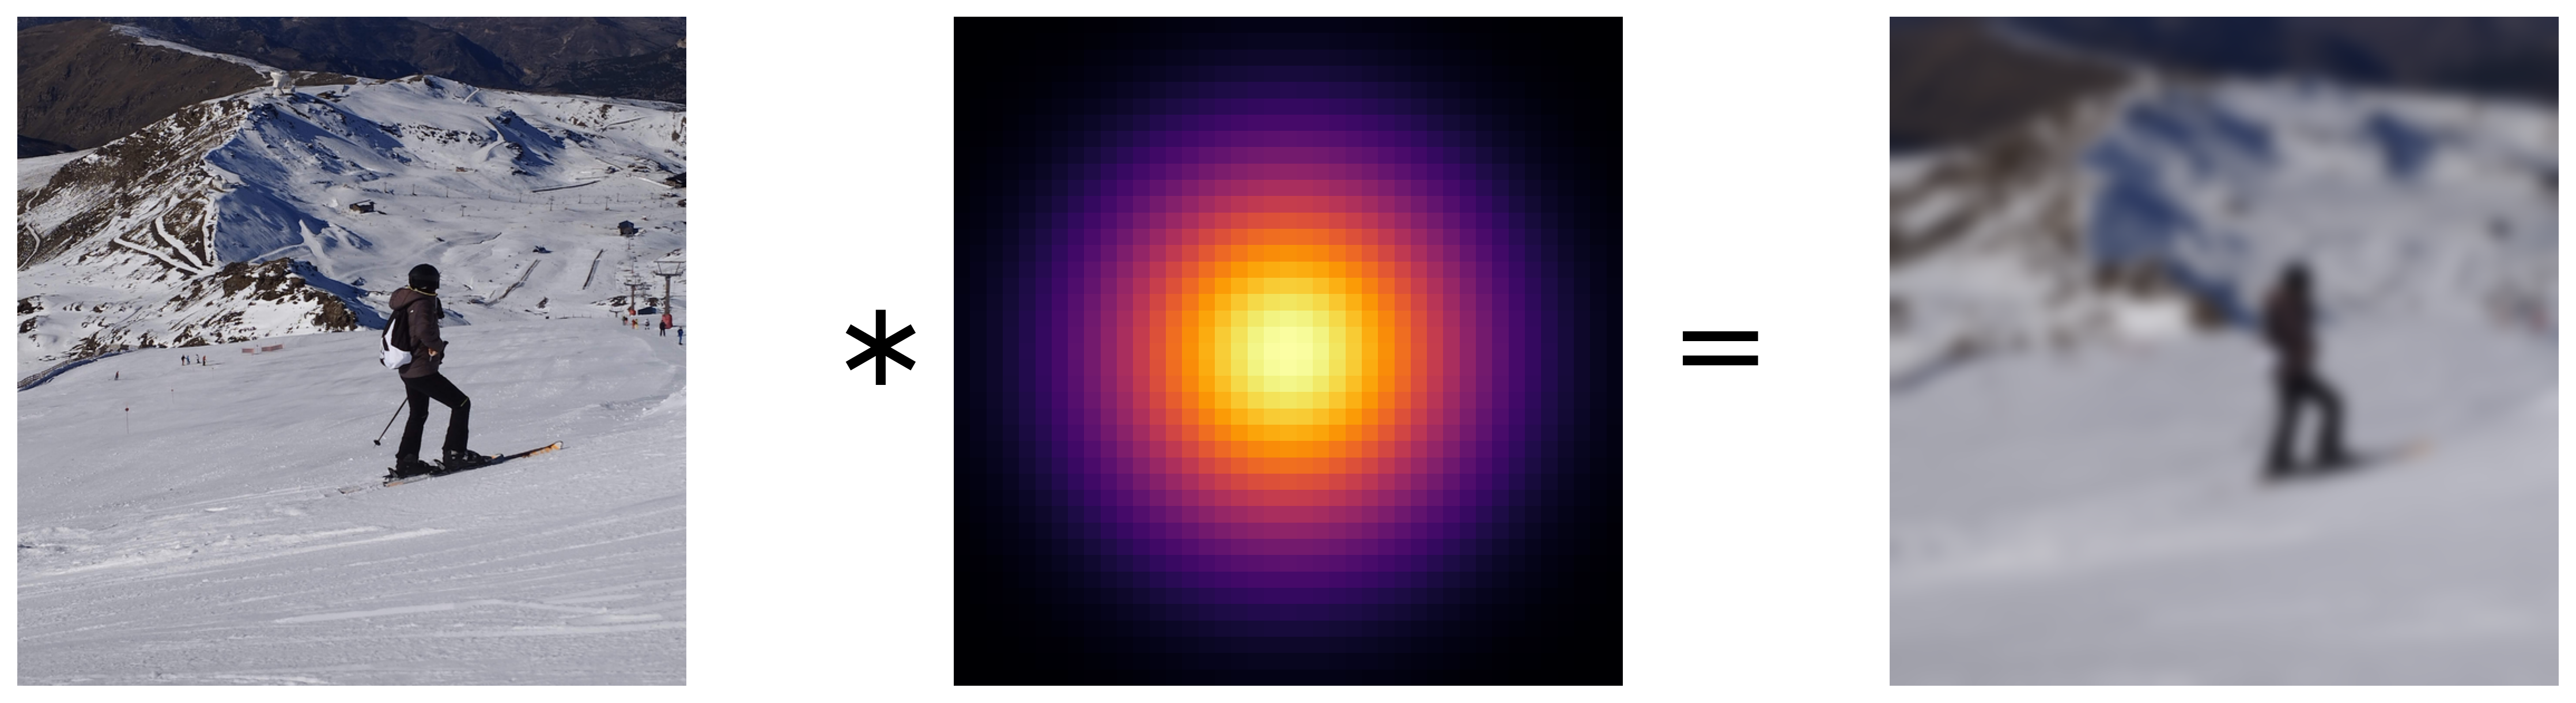
\includegraphics[width=0.8\textwidth]{img/ejemplo_degradacion.png}
    \caption{En esta imagen se muestra un ejemplo de cómo una imagen real se degrada al pasar por una lente. Se muestra de izquierda a derecha la imagen real ($d_{real}$), la PSF de la lente ($p$), y la imagen observada ($d_{observado}$).}
    \label{fig:ejemploConvolucion}
\end{figure}


Para hacer que este problema matemático sea más manejable, la técnica habitual es aplicar la Transformada de Fourier bidimensional. Esto nos permite pasar del dominio de la posición al dominio de las frecuencias espaciales. Si lo pensamos físicamente, estas frecuencias nos dicen cómo de rápido cambia la intensidad de la luz a lo largo de la imagen. Por ejemplo, las zonas donde la iluminación cambia poco a poco son las bajas frecuencias, mientras que los bordes marcados o los detalles más finos corresponden a las altas frecuencias. La gran ventaja matemática de saltar a este dominio es el Teorema de Convolución: gracias a él, una operación tan pesada como la convolución se convierte en una simple multiplicación, y viceversa.

\begin{equation}
    \label{eq:propFurier}
    \begin{split}
        \cdot &\Longrightarrow * \\
        * &\Longrightarrow \cdot
    \end{split}
\end{equation}

Sabiendo esto, si aplicamos la transformada a nuestra ecuación inicial (\ref{eq:convolucion}), el modelo en frecuencias queda mucho más limpio:

\begin{equation}
    \label{eq:convolucionFourier}
    D_{observado} = D_{real} \cdot P
\end{equation}

En este texto, la convención de notación emplea letras minúsculas para el dominio espacial y mayúsculas para el dominio de las frecuencias espaciales.

Si estuviéramos en un caso puramente ideal, bastaría con despejar directamente para encontrar $d_{real}$. Solo tendríamos que dividir la transformada de la imagen observada entre la de la PSF, llegando a la siguiente ecuación:

\begin{equation}
    \label{eq:deconvolucionIdeal}
    D_{real} = \frac{D_{observado}}{P}
\end{equation}

Finalmente, bastaría con deshacer la transformada (aplicar la inversa) para recuperar nuestra imagen $d_{real}$. Sin embargo, la realidad es bastante distinta, ya que las observaciones reales siempre arrastran ruido. Por ello, el modelo completo tiene que incluir este nuevo factor:

\begin{equation}
    \label{eq:convolucionRuido}
    d_{observado} = d_{real} * p + n
\end{equation}

donde $n$ representa el ruido añadido por el detector, la atmósfera u otras fuentes instrumentales. Al pasar al dominio de Fourier, la expresión queda:

\begin{equation}
    \label{eq:convolucionFourierRuido}
    D_{observado} = D_{real} \cdot P + N
\end{equation}

Con el ruido presente, la idea de despejar dividiendo directamente se vuelve inestable. El motivo es que al dividir entre $P$, también acabamos amplificando el ruido:

\begin{equation}
    \label{eq:deconvolucionRuido}
    D_{real} = \frac{D_{observado} - N}{P}
\end{equation}

Por tanto, la calidad de la deconvolución depende fuertemente de la relación señal-ruido.

% !TeX root = ../main.tex

\section{Métodos de deconvolución: Fourier, Wiener y Richardson-Lucy}
\subsection{Deconvolución de Fourier}
El primer método utilizado lo he denominado método de Fourier. Este es el método presentado anteriormente en la sección anterior, presentado mediante la ecuación (\ref{eq:deconvolucionIdeal}). Entonces, para recordar el método, este se demuestra en los siguientes pasos. Si tenemos una imagen observada $d_{observado}$, y conocemos la PSF del telescopio $p$ (recordando la notación de minuscula para el dominio de las posiciones, y mayúscula para el dominio de las frecuencias espaciales), entonces:

\begin{enumerate}
    \item Se realiza la transformada de Fourier de la imagen observada y de la PSF, obteniendo así $D_{observado}$ y $P$.
    \item Se realiza la división de $D_{observado}$ entre $P$, obteniendo así $D_{real}$, tal y como se indica en la ecuación (\ref{eq:deconvolucionIdeal}).
    \item Se realiza la transformada de Fourier inversa para obtener el $d_{real}$.
\end{enumerate}

El problema de este método reside en que al dividir la imagen entre la PSF, el ruido presente en la imagen se puede amplificar, y por lo tanto el resultado puede ser inestable. Como se demostrará más adelante en el trabajo, este método no da buenos resultados. Por lo tanto tenemos que encontrar distintos métodos que nos sirvan para poder deconvolucionar la imagen tratando este ruido.

\subsection{Filtro de Wiener}

Como se ha demostrado anteriormente, la deconvolución mediante división directa en el dominio de Fourier falla drásticamente en presencia de ruido. Esto ocurre porque en las altas frecuencias espaciales los valores de la función de transferencia óptica tienden a cero, lo que provoca que al dividir por ellos, el ruido de alta frecuencia se amplifique desproporcionadamente y destruya la información de la imagen. 

Para solucionar este problema, se implementa el filtro de Wiener. Este método consiste en una técnica de filtrado lineal óptimo que busca minimizar el error cuadrático medio entre la imagen real estimada y la imagen original sin degradar. A diferencia del filtro inverso, el filtro de Wiener logra un equilibrio: actúa como una deconvolución normal en las frecuencias donde la señal es fuerte, pero atenúa fuertemente aquellas frecuencias donde el ruido domina.

El filtro de Wiener se aplica de forma algorítmica directamente en el dominio de las frecuencias espaciales. El procedimiento consiste en calcular la Transformada de Fourier de la imagen observada y multiplicarla por la función de transferencia del filtro. Matemáticamente, partiendo del modelo con ruido de la ecuación (\ref{eq:convolucionRuido}), la estimación de la imagen real $D_{real}(u,v)$ se define como \cite[cap. 5]{gonzalezDigitalImageProcessing2018}:

\begin{equation}
    D_{real}(u,v) = \left[ \frac{P^*(u,v)}{|P(u,v)|^2 + \frac{S_n(u,v)}{S_d(u,v)}} \right] D_{observado}(u,v)
\end{equation}

Donde $P(u,v)$ es la transformada de Fourier de la PSF, $P^*(u,v)$ es su complejo conjugado, y los términos $S_n(u,v)$ y $S_d(u,v)$ representan los espectros de potencia del ruido y de la señal, respectivamente. 

En el procesado de datos reales, los espectros de potencia exactos rara vez se conocen a priori. Por ello, es una práctica estándar en la implementación computacional aproximar el cociente de los espectros por una constante relacionada con la relación señal-ruido (SNR). Sustituyendo este término por $1/\mathrm{SNR}^2$, la expresión final implementada en el código para construir el filtro $W(u,v)$ resulta ser:

\begin{equation}
    W(u,v) = \frac{P^*(u,v)}{|P(u,v)|^2 + \frac{1}{\mathrm{SNR}^2} + \epsilon}
\end{equation}

Cabe destacar que se introduce el parámetro numérico $\epsilon$ en el denominador para garantizar la estabilidad del algoritmo y evitar posibles singularidades o divisiones por cero durante la ejecución computacional. \\


Analizando el comportamiento asintótico de la ecuación (4.2), se distinguen dos regímenes principales. En el rango de las bajas frecuencias espaciales, donde típicamente se concentra la mayor parte de la señal de las estructuras observadas, la relación señal-ruido ($\mathrm{SNR}$) toma valores elevados. En consecuencia, el término $1/\mathrm{SNR}^2$ tiende a cero y el filtro se aproxima al comportamiento de un filtro inverso clásico. Por el contrario, en el régimen de altas frecuencias espaciales, que suele estar dominado por las fluctuaciones rápidas del ruido instrumental, la $\mathrm{SNR}$ decae significativamente. Esto provoca que el denominador de la expresión aumente, atenuando así los componentes frecuenciales correspondientes y evitando la amplificación del ruido. \\

Para la implementación computacional de este filtro, ha sido necesario estimar numéricamente un valor global de $\mathrm{SNR}$ directamente a partir de la imagen observada. Para ello, se ha desarrollado una rutina empírica basada en el análisis estadístico de los píxeles adyacentes, estructurada en los siguientes pasos:

\begin{enumerate}
    \item \textbf{Estimación de la señal:} Se aproxima la amplitud característica de la señal mediante el cálculo del valor medio de intensidad de todos los píxeles que conforman la matriz de la imagen.
    
    \item \textbf{Extracción de la componente de ruido:} Se calcula la diferencia de intensidad entre columnas adyacentes de la imagen. Dado que las estructuras físicas reales presentan variaciones espaciales suaves a la escala de un píxel, esta sustracción cancela la mayor parte de la señal subyacente, aislando fundamentalmente las fluctuaciones de alta frecuencia asociadas al ruido aleatorio.
    
    \item \textbf{Cuantificación del nivel de ruido:} Asumiendo que el ruido en píxeles contiguos se comporta como variables aleatorias independientes, por las propiedades estadísticas de la varianza, la varianza de la diferencia de estas dos variables es igual a la suma de sus respectivas varianzas. Por tanto, la desviación típica de esta matriz diferencia será $\sqrt{2}$ veces mayor que la del ruido original de la imagen. Así, la estimación real del ruido se obtiene calculando la desviación estándar estadística de estas diferencias y dividiéndola por el factor de corrección $\sqrt{2}$.
\end{enumerate}

Finalmente, la estimación de la $\mathrm{SNR}$ que se introduce en el algoritmo de deconvolución se obtiene como el cociente directo entre el valor medio de la señal y esta estimación estadística del ruido.

\subsection{Algoritmo de Richardson-Lucy}

A diferencia de los métodos de Fourier y Wiener, que resuelven el problema de forma directa usando las frecuencias, el algoritmo de Richardson-Lucy funciona mediante iteraciones. Este método asume que el ruido de la imagen sigue una estadística de Poisson, lo cual viene muy bien para imágenes astronómicas que se basan en contar fotones.

La principal ventaja de este método es que asegura que los píxeles de la imagen resultante sean siempre positivos (siempre que la original y la PSF también lo sean) y mantiene el flujo total de energía de la imagen. La ecuación iterativa del método es la siguiente \cite{richardsonBayesianBasedIterativeMethod1972}:

\begin{equation}
    u^{(k+1)} = u^{(k)} \cdot \left( \frac{d_{observado}}{u^{(k)} \ast p} \ast p^* \right)
\end{equation}

Donde $u^{(k)}$ es la imagen que se estima en la iteración $k$, $d_{observado}$ es la imagen observada, $p$ es la PSF y $p^*$ es la PSF girada o invertida. Además, el símbolo $\ast$ indica que se trata de una convolución.

Para implementar esto en el código, el algoritmo hace los siguientes pasos repetidas veces para ir mejorando la imagen:

\begin{enumerate}
    \item Primero se convoluciona la estimación que se tiene de la imagen con la PSF normal ($u^{(k)} \ast p$). Con esto se simula cómo se vería esa estimación si pasara de verdad por el telescopio. Al igual que antes, se le suma un número muy pequeño ($\epsilon = 10^{-12}$) para no tener divisiones por cero.
    \item Después se divide la imagen observada ($d_{observado}$) entre la imagen simulada del paso anterior. Si la estimación fuera perfecta, esta división daría exactamente 1 en todos los píxeles.
    \item Luego se convoluciona ese resultado con la PSF girada. Con esto se calcula la corrección que hay que aplicar.
    \item Por último, se multiplica la estimación actual ($u^{(k)}$) por esa corrección que se ha calculado para obtener la nueva estimación ($u^{(k+1)}$) del siguiente paso.
\end{enumerate}

Este proceso se va repitiendo un número determinado de veces, que en el código se controla con la variable \textit{pasos} (por defecto se ha puesto a 30). El mayor problema de usar este método es que no tiene un punto claro donde parar por sí solo. Si se hacen demasiadas iteraciones, el algoritmo intenta ajustar también el ruido de fondo, amplificándolo y creando pequeños artefactos (como puntos o ruido) por la imagen. \\

Otro problema que se ha comentado anteriormente, el algoritmo solo detecta señales positivas. Por lo tanto es inválido para señales que contengan valores tanto positivos como negativos. Es el caso de la señal de Stokes $V$, que es necesario deconvolucionar para poder extraer el campo magnético. Pero aún así, como se indicará más adelante, este es el método con mejores resultados para la intensidad de los tres, por lo que es el utilizado. \\

Otro detalle a destacar de los dos últimos métodos es el uso del padding. Al realizar la convolución, los píxeles de los bordes de la imagen se ven afectados por el hecho de que no hay información fuera de la imagen. Para evitar esto, se añade un borde del tamaño de la PSF alrededor de la imagen, rellenando ese borde con un espejo de la imagen. De esta forma, al realizar la convolución, los píxeles de los bordes se ven afectados por un reflejo de la imagen y no por ceros, lo que hace que el resultado sea más estable en los bordes y se obtenga un mejor resultado. Al final, se recorta la imagen para quedarse solo con la parte original y no con el padding.

\subsection{El problema de la deconvolución del campo magnético}

El problema central de este trabajo surge al analizar la ecuación de aproximación de campo débil (\ref{eq:campoDebil}). Experimentalmente, lo que se miden son los parámetros de Stokes $V$ e $I$. Como dijimos antes, la deconvolución de $V$ no es fácil debido a que tiene componente negativa.

Al expresar matemáticamente la señal observada afectada por la degradación instrumental (modelada mediante la convolución con la PSF), e introducimos la ecuación de aproximación de campo débil (\ref{eq:campoDebil}), obtenemos la siguiente expresión:

\begin{equation}
    \label{eq:expresionConvolucionada}
    V_{\mathrm{obs}} = V \ast \mathrm{PSF} = \left(-C g_{\mathrm{eff}} \lambda^2 B_{\parallel} \frac{d I_0}{d \lambda} \right) \ast \mathrm{PSF}
\end{equation}

Como se puede observar al expandir la expresión, el campo magnético longitudinal $B_{\parallel}$ que intentamos extraer multiplica a la derivada de la intensidad antes de que se aplique la convolución espacial. Recordando las propiedades presentadas en (\ref{eq:propFurier}), el problema fundamental radica en la siguiente desigualdad:

\begin{equation}
    \label{eq:imposibilidadDecon}
    \left(-C g_{\mathrm{eff}} \lambda^2 B_{\parallel}(x, y) \frac{d I_0}{d \lambda}(x, y) \right) \ast \mathrm{PSF} \neq -C g_{\mathrm{eff}} \lambda^2 \left(B_{\parallel}(x, y) \ast \mathrm{PSF} \right) \left(\frac{d I_0}{d \lambda}(x, y) \ast \mathrm{PSF} \right)
\end{equation}

Esto se debe a que el operador de convolución no es distributivo respecto al producto de funciones, lo que imposibilita la deconvolución trivial y el aislamiento directo del término del campo magnético.



% !TeX root = ../main.tex

\section{Método de Van Noort y método desarrollado}
A continuación, se expone el método original desarrollado en este trabajo para aislar y extraer el campo magnético a partir de las señales observables de Stokes $V$ e $I$. El núcleo de esta aportación se fundamenta en la teoría matemática propuesta por Van Noort \cite{vannoortSpatiallyCoupledInversion2012}, la cual ha sido adaptada e implementada específicamente para resolver el problema de la convolución que nos ocupa.

El marco teórico original introducido por Van Noort se articula del siguiente modo. Supóngase un conjunto de datos observacionales $d$ y un modelo analítico predictivo $F(x)$ dependiente de un vector de parámetros $x$ (en el contexto de este estudio, el modelo corresponde a la aproximación de campo débil y el parámetro es el campo magnético longitudinal). Dada una estimación inicial de los parámetros, denotada como $x_0$, el vector residual o error se define como:

\begin{equation}
    \label{eq:beta}
    \beta = d -F(x_0)
\end{equation}

Para optimizar esta estimación inicial, se busca determinar un vector de corrección $\nu$, de manera que la nueva aproximación actualizada se exprese como $x_0 + \nu$.

Dado que, según la formulación original, la función $F(x)$ es típicamente compleja y no lineal, se procede a linealizarla mediante una expansión en serie de Taylor de primer orden:

\begin{equation}
    F(x_o + \nu) \simeq F(x_0) + J \nu
\end{equation}

donde $J$ es la matriz Jacobiana del sistema. 

La convergencia ideal del algoritmo exige que la nueva estimación concuerde analíticamente con los datos observados, anulando el residuo:

\begin{equation}
    \begin{split}
        d - F(x_o + \nu) &= 0\\
        d - (F(x_0) + J \nu) &= 0\\
        J \nu = \beta
    \end{split}
\end{equation}

donde $\beta = d - F(x_0)$. La dificultad analítica subyacente en el tratamiento de datos experimentales radica en que el número de observaciones supera ampliamente al de parámetros libres a ajustar. En consecuencia, $J$ adquiere la estructura de una matriz rectangular, configurando un sistema algebraico sobredeterminado. 

Para abordar la resolución de este sistema, se implementa una formulación de mínimos cuadrados. Siguiendo la derivación del autor original, la optimización cuadrática del residuo conduce al siguiente sistema de ecuaciones normales:

\begin{equation}
    \label{eq:sistemaResolver}
    J^T J \nu = J^T \beta
\end{equation}

Esta reformulación algebraica permite calcular la corrección, dado que el producto matricial $J^T J$ genera una matriz cuadrada e invertible. Además, la arquitectura del método integra restricciones físicas intrínsecas del sistema para favorecer la convergencia hacia soluciones físicamente viables.

\subsection{Adaptación de la metodología al problema de la convolución polarimétrica}
La matriz $J$ representa el Jacobiano del sistema físico. En este TFG, el modelo directo consta de dos pasos: el cálculo local de la señal de polarización bajo la aproximación de campo débil y su posterior degradación espacial al convolucionar con la PSF. Como cada parámetro $x_i$ está asociado a un píxel de la imagen original, el tamaño del problema bidimensional se dispara. Para imágenes de 1400x1400 píxeles, calcular y almacenar explícitamente la matriz Jacobiana resulta inviable por falta de memoria RAM.

En este punto es donde reside la principal optimización de este método. En lugar de construir $J$ explícitamente como una matriz gigantesca, podemos tratarla matemáticamente como un operador lineal. Esta linealidad garantiza la existencia de su operador adjunto (o transpuesto) $J^T$, lo que permite resolver el sistema (\ref{eq:sistemaResolver}) de forma iterativa sin necesidad de almacenar la matriz en memoria.

Para demostrar esta linealidad, partimos de la aproximación de campo débil (\ref{eq:campoDebil}) y agrupamos todos los términos que no dependen del campo magnético en un único factor espacial $K(x, y, \lambda)$:

\begin{equation}
    V = - C \bar{g} \lambda_B^2 \frac{dI_0}{d \lambda} B_{\parallel} = K(x, y, \lambda) B_{\parallel}
\end{equation}

De este modo, la variación de los datos observados respecto al parámetro libre (el campo $B_{\parallel}$) equivale a multiplicar por el factor $K$ y, a continuación, aplicar la convolución espacial. Como tanto la derivada como la convolución son operadores lineales, el Jacobiano se puede expresar funcionalmente como:

\begin{equation}
    \label{eq:demosLinealidad}
    J = \frac{\partial V_{obs}}{\partial B_{\parallel}} = \frac{\partial}{\partial B_{\parallel}} \left[(K \cdot B_{\parallel}) * P \right] = \left[\frac{\partial}{\partial B_{\parallel}} (K \cdot B_{\parallel})\right] * P = K * P
\end{equation}

Al confirmar que $J$ es un operador lineal, queda garantizada la existencia de su operador traspuesto $J^T$, definido mediante el producto escalar estándar $\langle \cdot , \cdot \rangle$. Para cualquier par de funciones $x$ e $y$, el traspuesto debe cumplir la identidad:

\begin{equation}
    \label{eq:defTraspuesta}
    \langle Jx , y \rangle = \langle x , J^T y \rangle
\end{equation}

Observando la ecuación (\ref{eq:demosLinealidad}), vemos que $J$ es la composición de dos operaciones: un operador de convolución $C_p$ y uno de multiplicación diagonal $M_k$. Como la multiplicación por un escalar es autoadjunta, su traspuesta es ella misma. Por tanto:

\begin{equation}
    \label{eq:defTraspuesConjunta}
    J^T = (C_p M_k)^T = M^T_k C_p^T = M_k C_p^T
\end{equation}

Por otro lado, es conocido que el adjunto de una convolución equivale a convolucionar con el núcleo invertido espacialmente (rotado $180^\circ$), que denotaremos como $\tilde{P}$. Con todo esto, la acción del operador Jacobiano traspuesto sobre un mapa de campo magnético queda definida en su forma definitiva:

\begin{equation}
    \label{eq:jacobianaTras}
    J^T B_{\parallel} = K \cdot (\tilde{P} \ast B_{\parallel})
\end{equation}

\subsection{Resolución numérica: Subespacios de Krylov y Gradiente Conjugado}

Sustituyendo el operador directo (\ref{eq:demosLinealidad}) y su traspuesto (\ref{eq:jacobianaTras}) en el sistema de ecuaciones normales (\ref{eq:sistemaResolver}), el problema se reduce a resolver un sistema lineal de la forma $Ax = b$. 

El esquema computacional del método es el siguiente:

\begin{figure}[H]
    \centering
    \begin{tikzpicture}[
        node distance=0.8cm,
        font=\small,
        block/.style={rectangle, draw, fill=purple!10, text width=6.5cm, text centered, rounded corners, minimum height=1cm},
        arrow/.style={-{Stealth[scale=1.0]}, thick}
        ]
        
        \node[block] (step1) {\textbf{1. Inicialización:} \\ Estimación inicial $B_{\parallel}^0$};
        \node[block, below=of step1] (step2) {\textbf{2. Modelo sintético:} \\ Señal $V' = J B_{\parallel}^0$};
        \node[block, below=of step2] (step3) {\textbf{3. Residuo:} \\ $\beta = V_{\mathrm{obs}} - V'$};
        \node[block, below=of step3] (step4) {\textbf{4. Corrección:} \\ Resolver $J^T J \Delta B_{\parallel} = J^T \beta$};
        
        \draw[arrow] (step1) -- (step2);
        \draw[arrow] (step2) -- (step3);
        \draw[arrow] (step3) -- (step4);
    \end{tikzpicture}
    \caption{Diagrama de flujo del esquema computacional del método de inversión.}
    \label{fig:flowchart_metodo}
\end{figure}

Este proceso da lugar a la siguiente ecuación de optimización:

\begin{equation}
    \label{eq:sistemaEcReal}
    J^T J \Delta B_{\parallel} = J^T \beta
\end{equation}

En la notación algebraica estándar, la matriz del sistema es $A = J^T J$, la incógnita a despejar es la corrección $x = \Delta B_{\parallel}$, y el término independiente es $b = J^T \beta$.

La resolución de este sistema proporciona el mapa bidimensional de correcciones $\Delta B_{\parallel}$, que se suma a la estimación inicial $B_{\parallel}^0$ para generar el mapa de campo magnético actualizado: $B_{\parallel}^f = B_{\parallel}^0 + \Delta B_{\parallel}$.

Dado que calcular y almacenar explícitamente la matriz $A$ sigue siendo inviable, plantear el problema mediante operadores lineales permite emplear métodos iterativos basados en subespacios de Krylov. La principal ventaja de esta familia de algoritmos es que solo requieren evaluar el producto de la matriz por un vector (en este caso, aplicar secuencialmente los operadores sobre la imagen), evitando por completo calcular y guardar los coeficientes de la matriz.

Dentro de los métodos de Krylov, y dado que nuestra matriz $J^T J$ es por construcción simétrica y definida positiva, el algoritmo idóneo para la resolución es el método del Gradiente Conjugado (CG). Este método construye iterativamente direcciones de búsqueda ortogonales (conjugadas) en el subespacio, minimizando el error de forma óptima en cada iteración. Al ser un algoritmo ampliamente estandarizado, su integración resulta directa empleando bibliotecas de cálculo científico convencionales.
% !TeX root = ../main.tex

\section{Métodos de análisis de resultados}
Para evaluar objetivamente los resultados de los algoritmos de deconvolución, se emplean dos parámetros métricos que permiten cuantificar la calidad de la reconstrucción utilizando datos sintéticos, dado que en estos casos se dispone de la señal original para su comparación directa. 

\subsection{Raíz del error cuadrático medio (RMSE)}
Este parámetro mide la magnitud promedio del error entre la señal original (ideal o de referencia) y otra señal distinta, ya sea la propia señal emborronada por el instrumento o la señal reconstruida tras aplicar un algoritmo de deconvolución. La ecuación que define esta métrica es la siguiente:

\begin{equation}
    \label{eq:RMSE}
    RMSE = \sqrt{\frac{1}{N}\sum_{i=1}^{N}(x_i - y_i)^2}
\end{equation}

donde $x_i$ es el valor de la señal original en el punto (o píxel) $i$, $y_i$ es el valor de la señal a comparar en ese mismo punto, y $N$ es el número total de elementos discretos de la señal. 

Dado que penaliza las diferencias elevándolas al cuadrado, un valor de RMSE más bajo indica que la señal recuperada es cuantitativamente más fiel a la señal original. Por el contrario, un RMSE más alto evidencia una mayor discrepancia entre la señal procesada y la referencia.

\subsection{Índice de Similitud Estructural (SSIM)}
El SSIM es una métrica de calidad de imagen que, a diferencia del RMSE, evalúa la degradación de la estructura espacial. Considera tres factores fundamentales: luminancia, contraste y estructura. El resultado de esta métrica es un valor comprendido entre $-1$ y $1$, donde los valores cercanos a $1$ indican una alta similitud con la imagen original. 

Aunque matemáticamente pueden presentarse valores negativos correspondientes a una correlación estructural inversa, la degradación instrumental estudiada no produce tales efectos. Por tanto, el rango de valores de interés físico para este análisis se restringe a $[0,1]$. 

Dada la complejidad analítica en el cálculo explícito de esta métrica, se recurre a la implementación computacional provista por la función \texttt{ssim} de la biblioteca \texttt{scikit-image} en Python, facilitando la evaluación eficiente del índice entre pares de imágenes. 

Cabe destacar que, si bien el RMSE y el SSIM proporcionan evaluaciones cuantitativas rigurosas, la inspección visual cualitativa de las imágenes sigue siendo un criterio complementario fundamental para dictaminar la viabilidad final de la reconstrucción.

% !TeX root = ../main.tex

\section{Análisis de resultados}

\subsection{Datos sintéticos}
Para empezar, trabajamos con unos datos sintéticos que simulan una zona del Sol en calma. El formato de estos datos es $[101,\,4,\,336,\,336]$, lo que significa que tenemos $101$ longitudes de onda, las $4$ componentes de Stokes ($I$, $Q$, $U$ y $V$) y un tamaño espacial de $336\times336$ píxeles. \\
Para poner a prueba los métodos de deconvolución, el primer paso fue emborronar artificialmente estas imágenes usando una PSF de tipo Airy. Esta función es una aproximación teórica de cómo se comporta un telescopio ideal cuya única limitación es tener una apertura circular. Matemáticamente, su perfil radial se escribe así:
\begin{equation}
    \label{eq:PSF}
    PSF(r) = I_0 \left(\frac{2 J_1(kr)}{kr} \right)
\end{equation}

donde $J_1$ es la función de Bessel de primer orden, $k$ es una constante que depende del diámetro del telescopio y de la longitud de onda, e $I_0$ es la intensidad máxima. 

En este caso se usa una PSF de 30 pixeles de radio y un tamaño de bulbo central de 3 pixeles, donde su representación visual es la siguiente:

\begin{figure}[H]
    \centering
    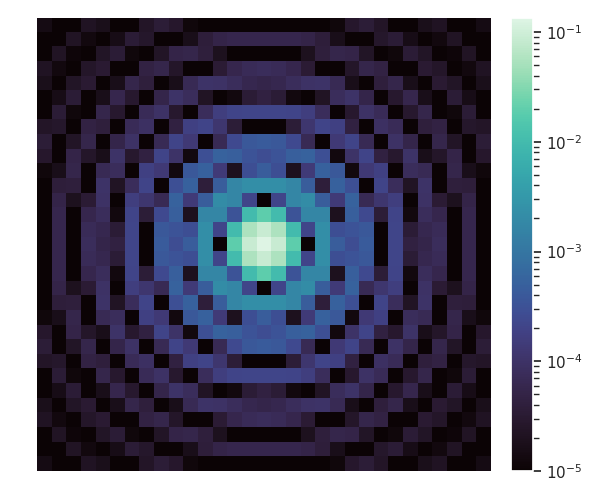
\includegraphics[width=0.7\textwidth]{img/comparacion_intensidad_4_psf.png}
    \caption{Esta imagen muestra la PSF de tipo Airy utilizada para emborronar la imagen original. Se puede observar que el bulbo central tiene un tamaño de 3 píxeles y que el radio de la PSF es de 30 píxeles. Esta representada en escala logaritmica para poder observar mejor la caída de la intensidad en los anillos de difracción.}
    \label{fig:psfAiry}
\end{figure}

Obviamente, para que la simulación sea realista, también necesitamos meter ruido en la ecuación. Añadimos ruido blanco gaussiano a cada componente de Stokes. Pero como la señal en el canal $I$ es muchísimo más fuerte que en el canal $V$, tuvimos que aplicar un esquema de ruido relativo. Esto significa que la desviación estándar ($\sigma$) del ruido se define como un porcentaje $p$ de la amplitud máxima de cada señal en particular, imitando mejor lo que ocurre en una observación real:
\begin{equation}
    I_{max} = \max(I(\mathbf{x})), \quad V_{max} = \max(|V(\mathbf{x})|)
\end{equation}
donde $\mathbf{x}$ representa las coordenadas espaciales y espectrales del cubo de datos. A partir de estos máximos, las desviaciones estándar para un porcentaje de ruido $p$ se definen como:
\begin{equation}
    \sigma_I = I_{max} \cdot \frac{p}{100}, \quad \sigma_V = V_{max} \cdot \frac{p}{100}
\end{equation}


\subsubsection{Análisis de los distintos métodos de deconvolución: Fourier, Wiener y Richardson-Lucy}

Primero se realizará una comparación visual entre los distintos métodos de deconvolución a partir de la Intensidad (primera componente de Stokes). Escogeremos una longitud de onda arbitraria y la emborronoramos con un ruido del $0.1 \%$. El resultado es el siguiente.



\begin{figure}[H]
    \centering
    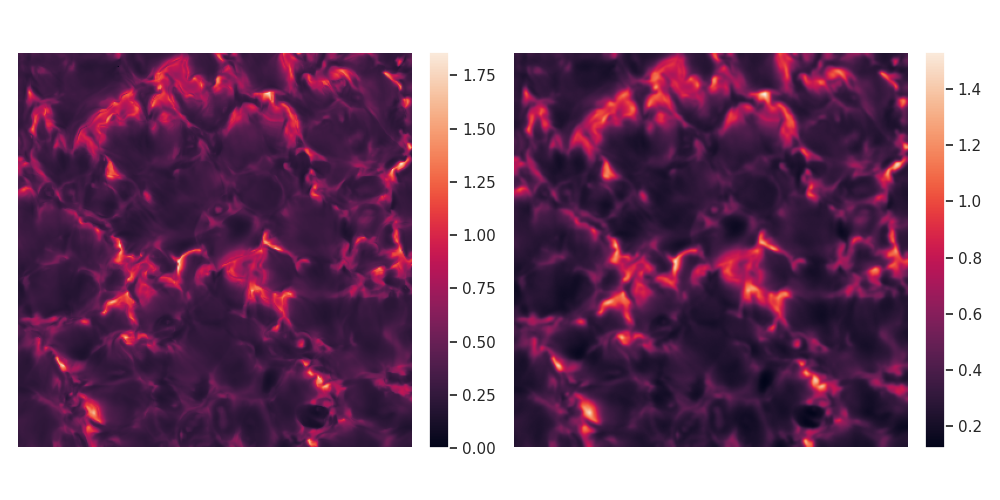
\includegraphics[width=0.9\textwidth]{img/comparacion_intensidad_1_original_borrosa.png}
    \caption{Esta imagen muestra dos mapas de intensidad. A la izquierda se muestra el mapar sintético original, mientras que a la derecha se muestra el mapa convolucionado con la PSF (\ref{fig:psfAiry}) y con un ruido del $0.1 \%$. Se puede observar que la imagen de la derecha está emborronada y que se han perdido detalles finos de la imagen original.}
    \label{fig:intensidadSintEmborro}
\end{figure}

Aunque se ve el emborronamiento, nos centraremos en una zona concreta de la imagen para observar mejor los detalles. Está representada en la siguiente figura:

\begin{figure}[H]
    \centering
    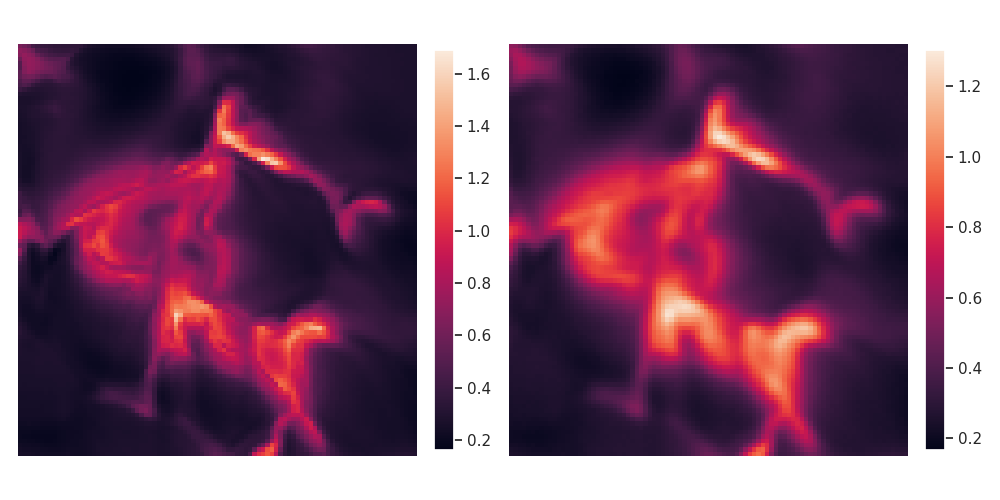
\includegraphics[width=0.9\textwidth]{img/comparacion_intensidad_5_original_borrosa_zoom.png}
    \caption{Región de la imagen de la figura \ref{fig:intensidadSintEmborro} donde se puede observar mejor el emborronamiento de la imagen. A la izquierda se muestra el mapa sintético original, mientras que a la derecha se muestra el mapa convolucionado con la PSF (\ref{fig:psfAiry}) y con un ruido del $0.1 \%$.}
    \label{fig:intensidadSintEmborroZoom}
\end{figure}

Entonces realizamos la deconvolución con los distintos métodos (Wiener, Fourier, Richardson-Lucy) y comparamos visualmente los resultados. El resultado es el siguiente:

\begin{figure}[H]
    \centering
    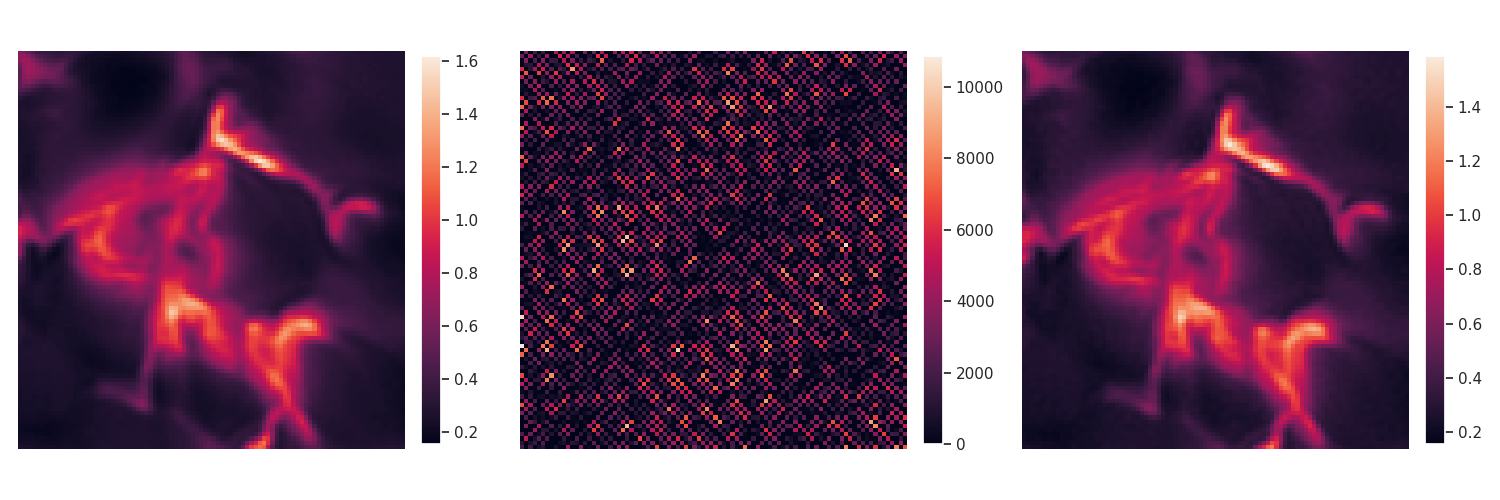
\includegraphics[width=1.0\textwidth]{img/comparacion_intensidad_6_deconvoluciones_zoom.png}
    \caption{Resultados de la deconvolución con los distintos métodos. A la izquierda se encuentra el mapa deconvolucionado con el método de Wiener, en el centro se encuentra el mapa deconvolucionado con el método de Fourier y a la derecha se encuentra el mapa deconvolucionado con el método de Richardson-Lucy.}
    \label{fig:deconvolucionClasicaZoom}
\end{figure}

Y si miramos los resultados de las métricas RMSE y SSIM, obtenemos los siguientes resultados:

\begin{figure}[H]
    \centering
    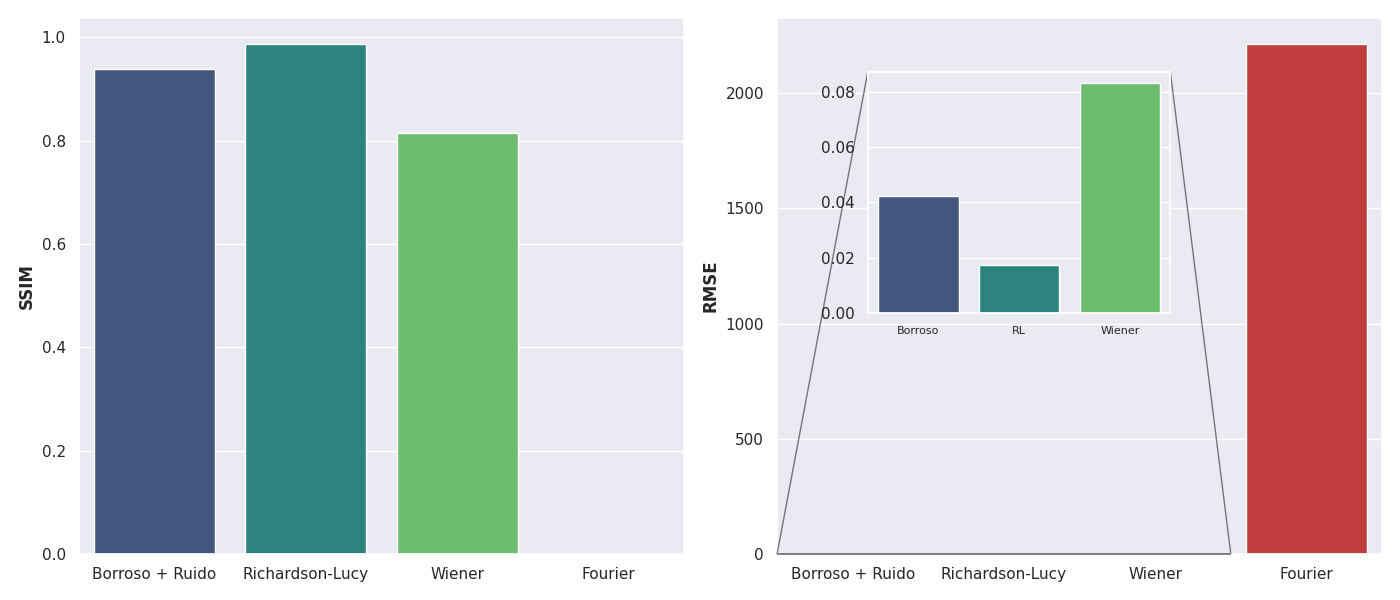
\includegraphics[width=1.0\textwidth]{img/comparacion_intensidad_3_barras.png}
    \caption{Valores de las métricas SSIM (izquierda) y RMSE (derecha) para los diferentes métodos de deconvolución. Se añade también la imagen emborronada para comparar sus valores. Debido al elevado valor de RMSE obtenido con el método de Fourier, la gráfica de la derecha incorpora una ampliación que permite apreciar con mayor detalle las diferencias entre el resto de métodos.}
    \label{fig:rsmeSsimIntensidad}
\end{figure}

Empezando por el método de Fourier, salta a la vista que sus métricas son desastrosas: tiene un SSIM casi nulo y un RMSE altísimo. Físicamente, esto se traduce en una imagen donde se ha perdido absolutamente todo el detalle. Como ya habíamos anticipado teóricamente, este método no soporta nada bien el ruido, quedando claro que no nos sirve para imágenes reales que no sean perfectas.

Si pasamos al filtro de Wiener, la situación es engañosa. Visualmente da la sensación de haber recuperado bastante detalle, pero si miramos los números, el SSIM es más bajo y el RMSE es más alto que los de la propia imagen emborronada sin tocar. Es decir, aunque a ojo parezca mejor, la reconstrucción real es peor. Seguramente esto pase porque hemos utilizado la versión más básica del filtro de Wiener; en la literatura actual hay versiones mucho más sofisticadas que logran corregir estos fallos (por ejemplo, \cite{orieuxBayesianEstimationRegularization2010}).

Por el contrario, el algoritmo de Richardson-Lucy es el claro ganador de esta comparativa. Consigue mejorar el SSIM y bajar el RMSE respecto a la imagen borrosa de partida. Demuestra ser mucho más robusto frente al ruido, y si miramos el resultado, es evidente cómo logra rescatar detalles finos que se habían emborronado por culpa de la PSF.

\subsubsection{Problema de la deconvolución de V}
Si analizamos como evoluciona la deconvolución de la señal de Stokes $V$, y lo analizamos a distintos porcentajes de ruido, obtenemos los siguientes resultados:

\begin{figure}[H]
    \centering
    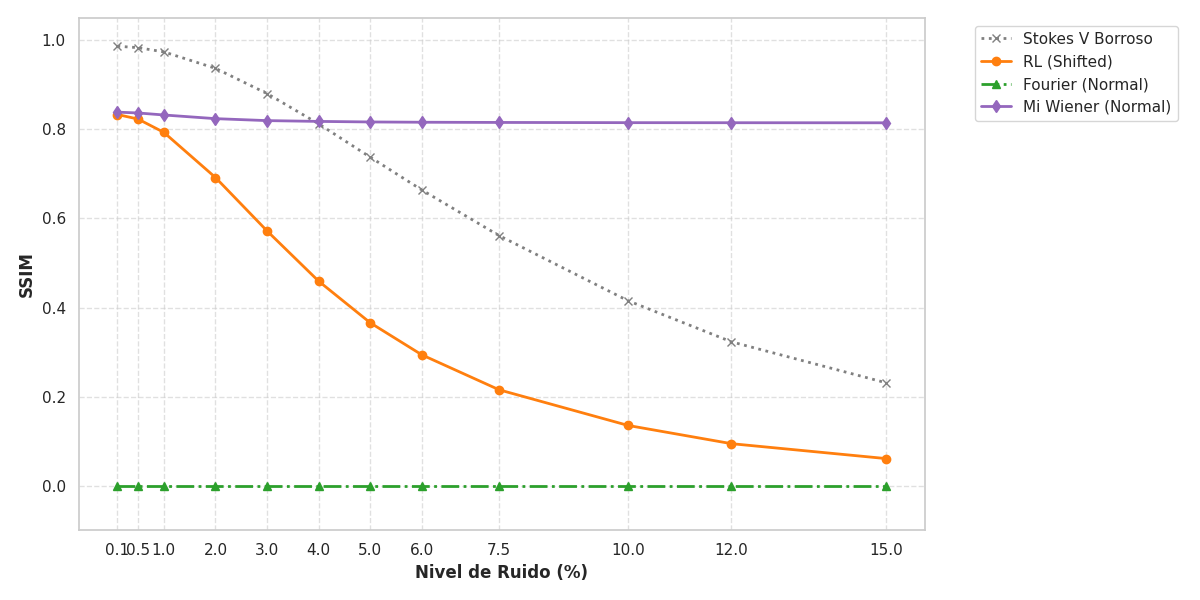
\includegraphics[width=1.0\textwidth]{img/experimento_stokesV_3_comparativa_shift.png}
    \caption{Evolución del SSIM en función del nivel de ruido para distintos métodos de deconvolución aplicados a la componente Stokes V. Se comparan los resultados de la imagen borrosa original frente a Richardson-Lucy (con \textit{shift} positivo), el filtro de Fourier y el filtro de Wiener.}
    \label{fig:SSIM_frenteARuidoV}
\end{figure}

Como la componente de Stokes $V$ tiene una amplitud tan pequeña, resulta extremadamente sensible al ruido. Esto provoca que ninguno de los algoritmos clásicos de deconvolución sea capaz de recuperar la señal original de forma satisfactoria. El método que ofrece mejores resultados es el filtro de Wiener. Para ilustrar este efecto, a continuación se muestra el mapa bidimensional recuperado por este filtro con un ruido del 2%:


\begin{figure}[H]
    \centering
    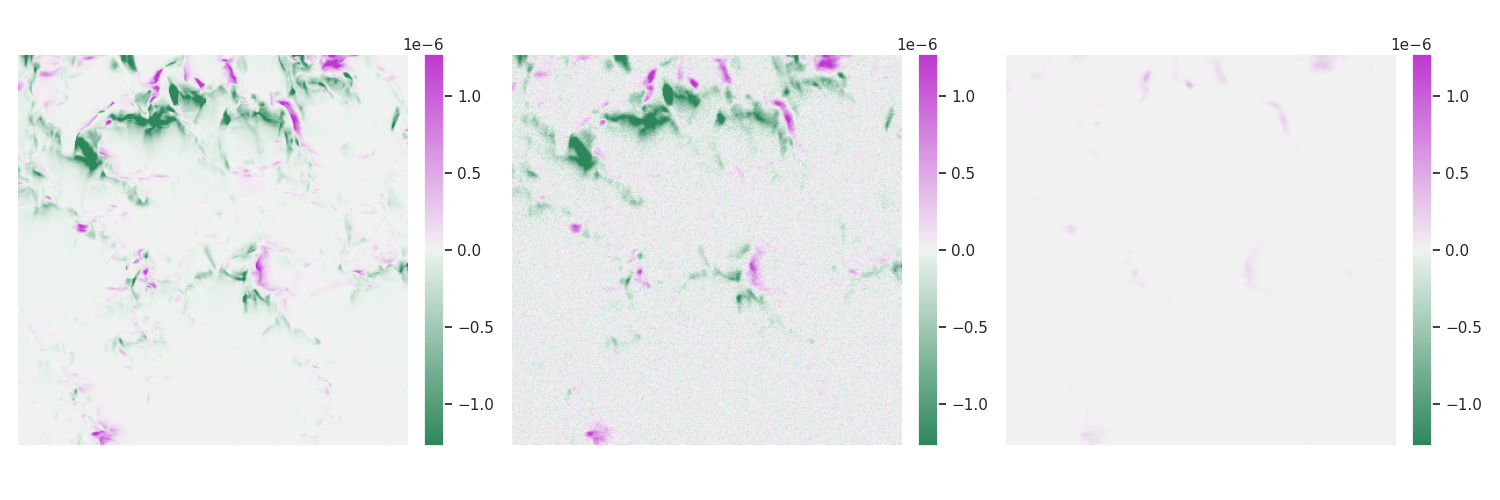
\includegraphics[width=1.0\textwidth]{img/experimento_stokesV_2_visualizacion.png}
    \caption{Comparativa visual de la componente Stokes V. De izquierda a derecha: mapa original (Ground Truth), mapa degradado con un $2\%$ de ruido, y resultado tras la deconvolución mediante el filtro de Wiener, mostrando el sobre-suavizado de la señal.}
    \label{fig:visualizacionStokesV}
\end{figure}

Esto explica por qué el índice SSIM se mantiene constante: el filtro de Wiener consigue eliminar el ruido, pero no logra recuperar la estructura de la señal original y termina suavizándola demasiado. 

Por lo tanto, este análisis demuestra que es inviable deconvolucionar la señal de Stokes $V$ con los métodos clásicos. Por esta razón, en este TFG se utiliza el método desarrollado para calcular el campo magnético directamente, evitando tener que deconvolucionar la señal de Stokes $V$.


\subsubsection{Método adaptado de Van Noort}
Antes de ver imágenes, vamos a comprobar si nuestro método converge como debería. Para ello, preparamos los datos igual que en el caso anterior: convolucionamos con la PSF y le metemos ruido. Como nuestra técnica es iterativa, va resolviendo el sistema poco a poco en cada paso. La mejor forma de asegurarnos de que todo marcha bien es vigilar el "residuo" tras cada iteración.

Ese residuo no es más que la diferencia entre lo que esperábamos obtener y la aproximación que ha logrado calcular el algoritmo en ese momento. Si medimos este error total (calculando la norma euclidiana $L_2$), obtenemos lo que llamamos diferencia iterativa. En la gráfica de abajo hemos representado esta evolución poniendo el eje vertical en escala logarítmica, lo que ayuda a ver muy claro cómo el error se desploma:

\begin{figure}[H]
    \centering
    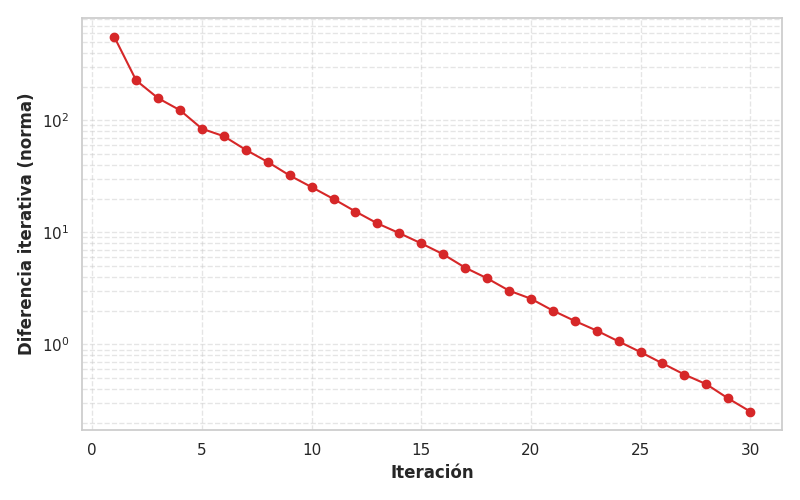
\includegraphics[width=0.8\textwidth]{img/experimento_noor_1_convergencia.png}
    \caption{Esta imagen muestra la evolución de la diferencia iterativa (la norma del residuo) a lo largo de las iteraciones del algoritmo de Noor. Se puede observar cómo el error va disminuyendo progresivamente, lo que indica que el método converge de forma correcta.}
    \label{fig:convergenciaNoor}
\end{figure}

Veremos entonces el resultado de esta deconvolución:

\begin{figure}[H]
    \centering
    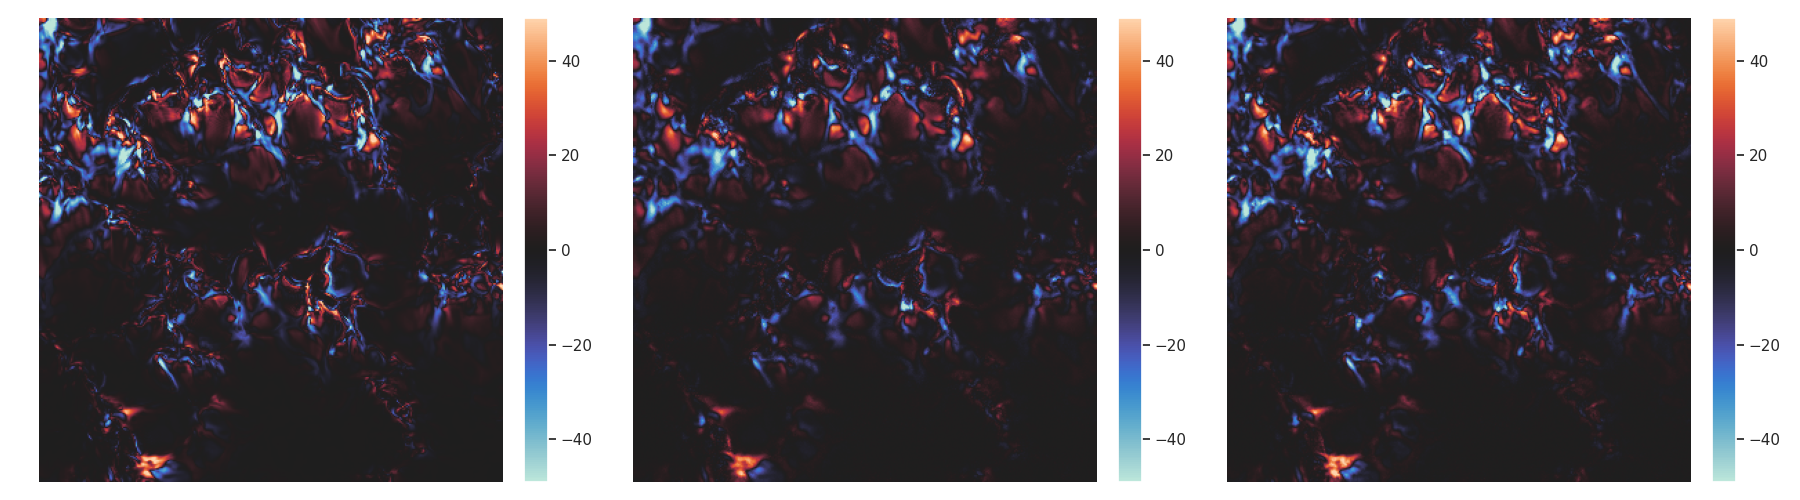
\includegraphics[width=1.0\textwidth]{img/experimento_noor_2_comparativa_b copy.png}
    \caption{Comparativa visual del campo magnético, representado en Gauss. De izquierda a derecha: mapa original (Ground Truth), mapa degradado con ruido, y resultado tras la deconvolución mediante el método adaptado de Noor.}
    \label{fig:campoMagDeco}
\end{figure}

Igual que antes, volveremos a hacer zoom a la misma zona de interes para observar mejor los detalles de la imagen. El resultado es el siguiente:

\begin{figure}[H]
    \centering
    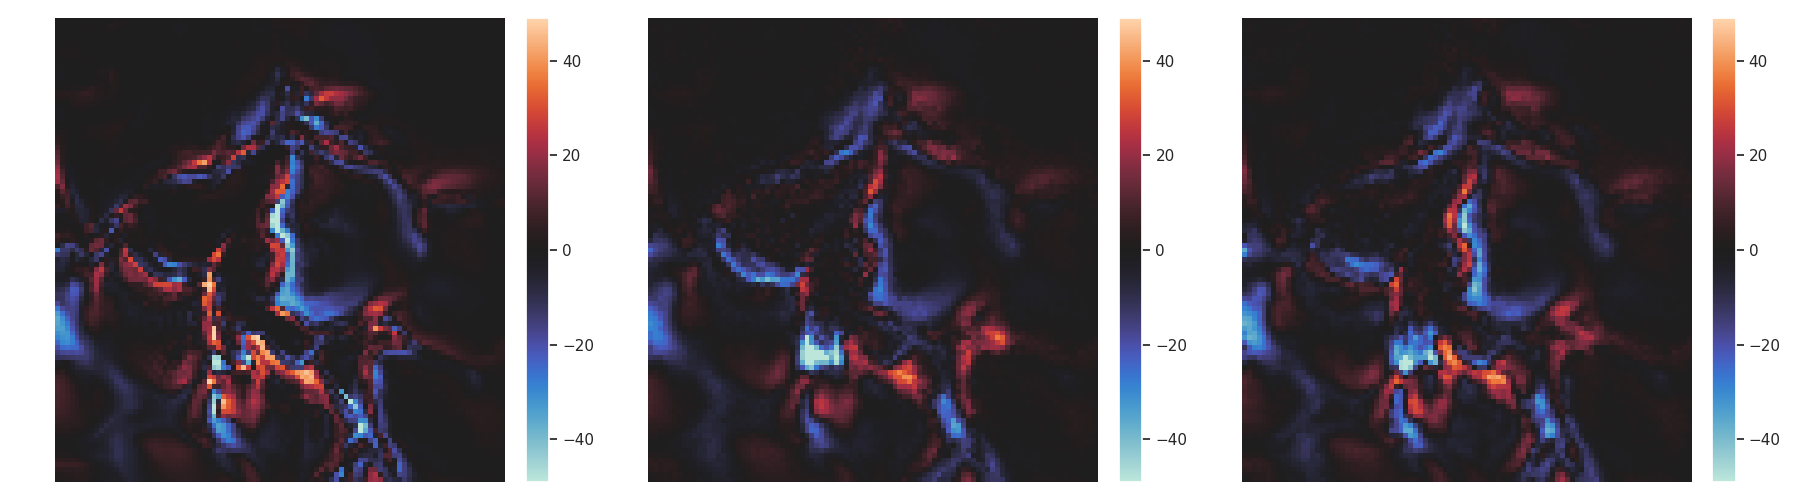
\includegraphics[width=1.0\textwidth]{img/experimento_noor_2b_comparativa_b_zoom.png}
    \caption{Comparativa visual del campo magnético, representado en Gauss. De izquierda a derecha: mapa original (Ground Truth), mapa degradado con ruido, y resultado tras la deconvolución mediante el método adaptado de Noor. Se puede observar que el método logra recuperar detalles finos del campo magnético que se habían perdido en la imagen degradada.}
    \label{fig:campoMagDecoZoom}
\end{figure}

Como salta a la vista, nuestro método consigue rescatar la estructura original del campo magnético. Las zonas vuelven a estar definidas e incluso recuperamos picos de intensidad que el emborronamiento se había "comido", lo cual es todo un éxito. Sí que es cierto que hay ciertos bulbos magnéticos que no quedan perfectos, pero es totalmente esperable: al emborronar la imagen físicamente perdimos parte de la información original, por lo que ningún método podrá inventársela. Salvando ese detalle, el resultado general es estupendo y confirma que nuestra técnica sí es capaz de extraer el campo magnético combinando las señales $I$ y $V$. 

Si miramos un mapa de diferencias entre la imagen original y borrosa, y la imagen original y la deconvolucionada, obtenemos el siguiente resultado:

\begin{figure}[H]
    \centering
    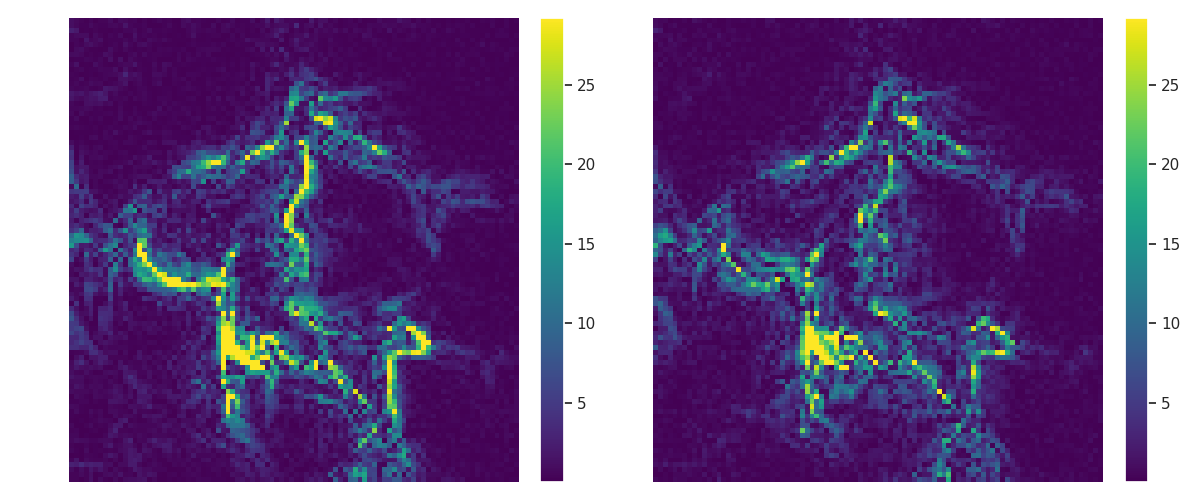
\includegraphics[width=1.0\textwidth]{img/experimento_noor_3b_residuos_zoom.png}
    \caption{Mapa de diferencias entre la imagen original y la degradada, y la imagen original y la deconvolucionada.}
    \label{fig:diferenciasZoom}
\end{figure}

Como vemos en la gráfica de diferencias, el residuo baja significativamente en las zonas de los filamentos, lo que demuestra que realmente está reconstruyendo la estructura. \\
Esta mejora que vemos a simple vista también la confirman los números. Nuestra imagen emborronada de partida tenía un SSIM de $0.8401$ y un RMSE de $5.2568$. Después de pasarle nuestro método adaptado de Van Noort (usando regularización de Laplace), el SSIM sube a $0.8575$ y el RMSE cae a $4.6995$. Matemáticamente, nos hemos acercado bastante más a la imagen ideal.

El siguiente paso natural es ver qué tal se porta el algoritmo cuando cambiamos los niveles de ruido. Hay que tener en cuenta que este método es bastante sensible al número de iteraciones: si nos pasamos dando pasos, acabaremos sobreajustando la señal y amplificando el ruido. El reto aquí es dar con el equilibrio perfecto entre cuántas iteraciones damos y cuánto ruido tiene la imagen. 

Para ello se realizó un estudio donde se encuentra el mejor SSIM y RMSE para distintos niveles de ruido, variando el número de iteraciones. Si vemos el mejor SSIM frente al nivel de ruido, obtenemos el siguiente resultado:

\begin{figure}[H]
    \centering
    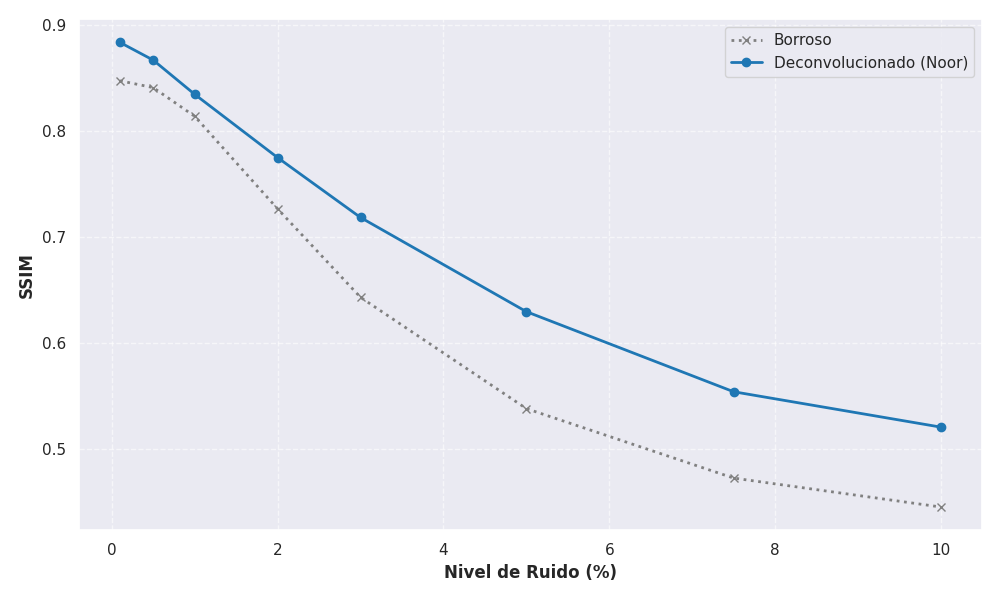
\includegraphics[width=0.7\textwidth]{img/experimento_noor_4_limite_ruido.png}
    \caption{Evolución del SSIM frente al nivel de ruido para el método adaptado de Noor. Se observa que el método siempre logra mejorar la imagen original.}
    \label{fig:SSIMfrenteARuidoNoor}
\end{figure}

Y si presentamos el mejor RMSE frente al nivel de ruido, obtenemos el siguiente resultado:

\begin{figure}[H]
    \centering
    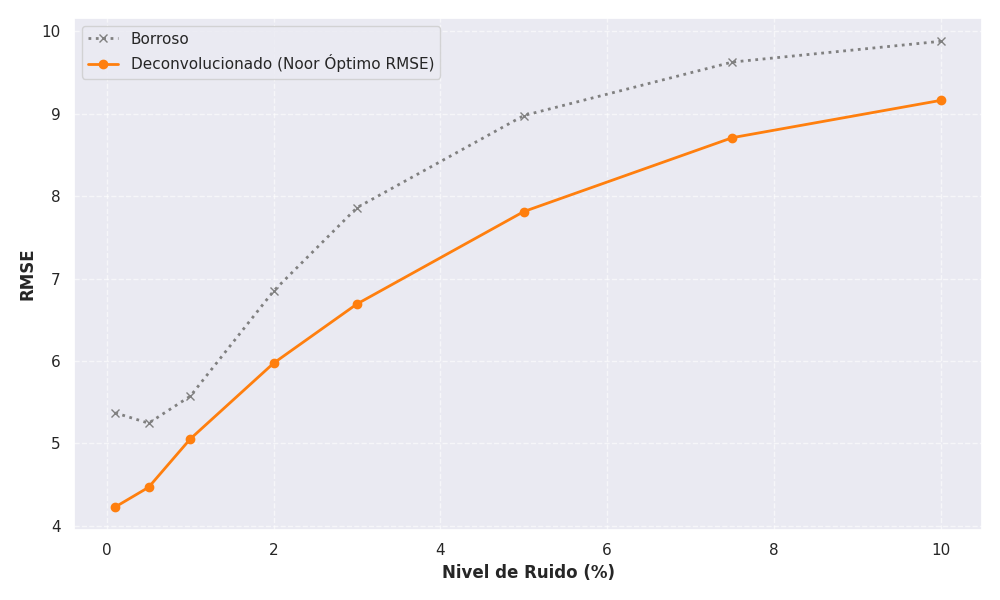
\includegraphics[width=0.7\textwidth]{img/experimento_noor_4b_limite_ruido_rmse.png}
    \caption{Evolución del RMSE frente al nivel de ruido para el método adaptado de Noor. Se observa que siempre es inferior.}
    \label{fig:RMSEfrenteARuidoNoor}
\end{figure}

Lo interesante de estas gráficas es ver que, sin importar cuánto ruido le echemos, el método siempre logra mejorar la imagen de partida. La clave de esto es que nuestro algoritmo no trabaja a ciegas; se apoya directamente en la física del problema para buscar una solución que encaje con la ecuación de transferencia radiativa. Gracias a esta restricción física, el método siempre es capaz de rascar algo de la señal original por mucho ruido que haya de fondo.

Si nos fijamos ahora en cuántas iteraciones hacen falta para dar con el mejor resultado en cada caso, llegamos a la siguiente gráfica:

\begin{figure}[H]
    \centering
    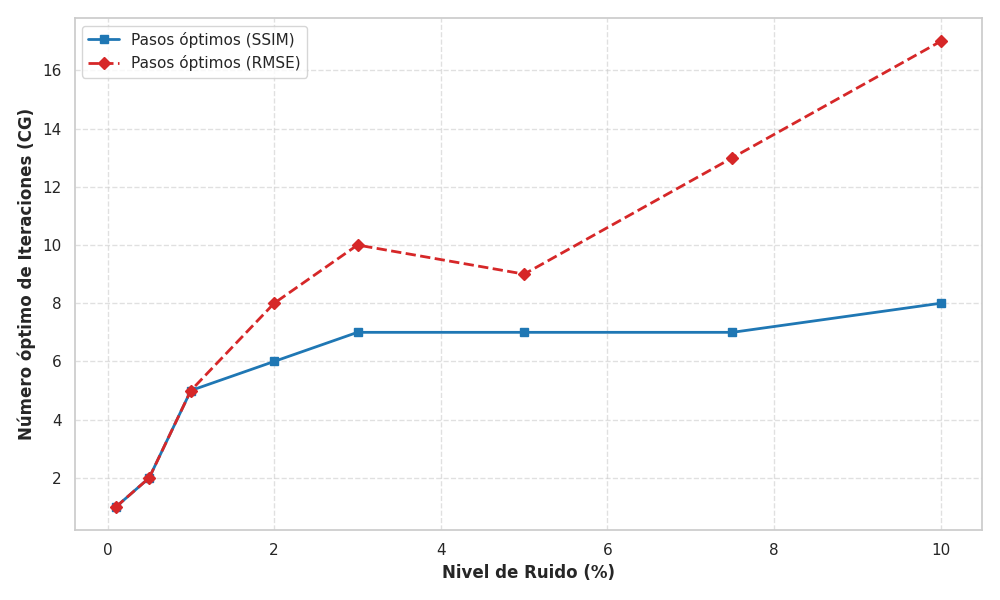
\includegraphics[width=0.7\textwidth]{img/experimento_noor_5_limite_ruido_pasos.png}
    \caption{Evolución del número de iteraciones frente al nivel de ruido para el método adaptado de Noor. La curva roja representa el numero de iteraciones para el valor de RMSE, y la curva azul representa el número de iteraciones para el valor de SSIM. Se observa que a medida que aumenta el nivel de ruido, se necesitan más iteraciones para conseguir el mejor resultado.}
    \label{fig:pasosfrenteARuidoNoor}
\end{figure}

Salta a la vista que siempre hacen falta más iteraciones para minimizar el RMSE que para alcanzar el mejor SSIM. Básicamente, el algoritmo necesita seguir iterando un rato más para limpiar el ruido estadístico (lo que mejora el RMSE), pero al hacerlo llega a un punto en el que empieza a emborronar ligeramente la estructura (lo que empeora el SSIM). Es el típico compromiso entre matar el ruido y conservar los bordes nítidos, algo parecido a lo que le pasaba a la componente $V$ en la figura (\ref{fig:visualizacionStokesV}).

\subsection{Datos reales} \label{sec:datosReales}
Ha llegado el momento de la verdad: probar todo esto con datos reales. Para ello, utilizamos las observaciones del experimento Sunrise-TUMAG disponibles públicamente \cite{SUNRISETuMagTUMAGData}. Concretamente, hemos cargado el archivo 
\begin{itemize}
    \item \textit{01\_QSUN\_TM\_00\_Mg1\_10\_10072024T131604\_LV\_1.0\_v0.4.fits}
\end{itemize}

Su estructura interna es $[10,\,4,\,1600,\,1600]$, lo que se traduce en 10 puntos de longitud de onda distintos, las 4 componentes de Stokes, y un mapa espacial enorme de $1600\times1600$ píxeles. 

El PSF fue cedido por el equipo de óptica de la sección de  física solar del IAA. Esta PSF se consiguió modelando computacionalmente la óptica del telescopio Sunrise, y se puede observar en la siguiente figura:

\begin{figure}[H]
    \centering
    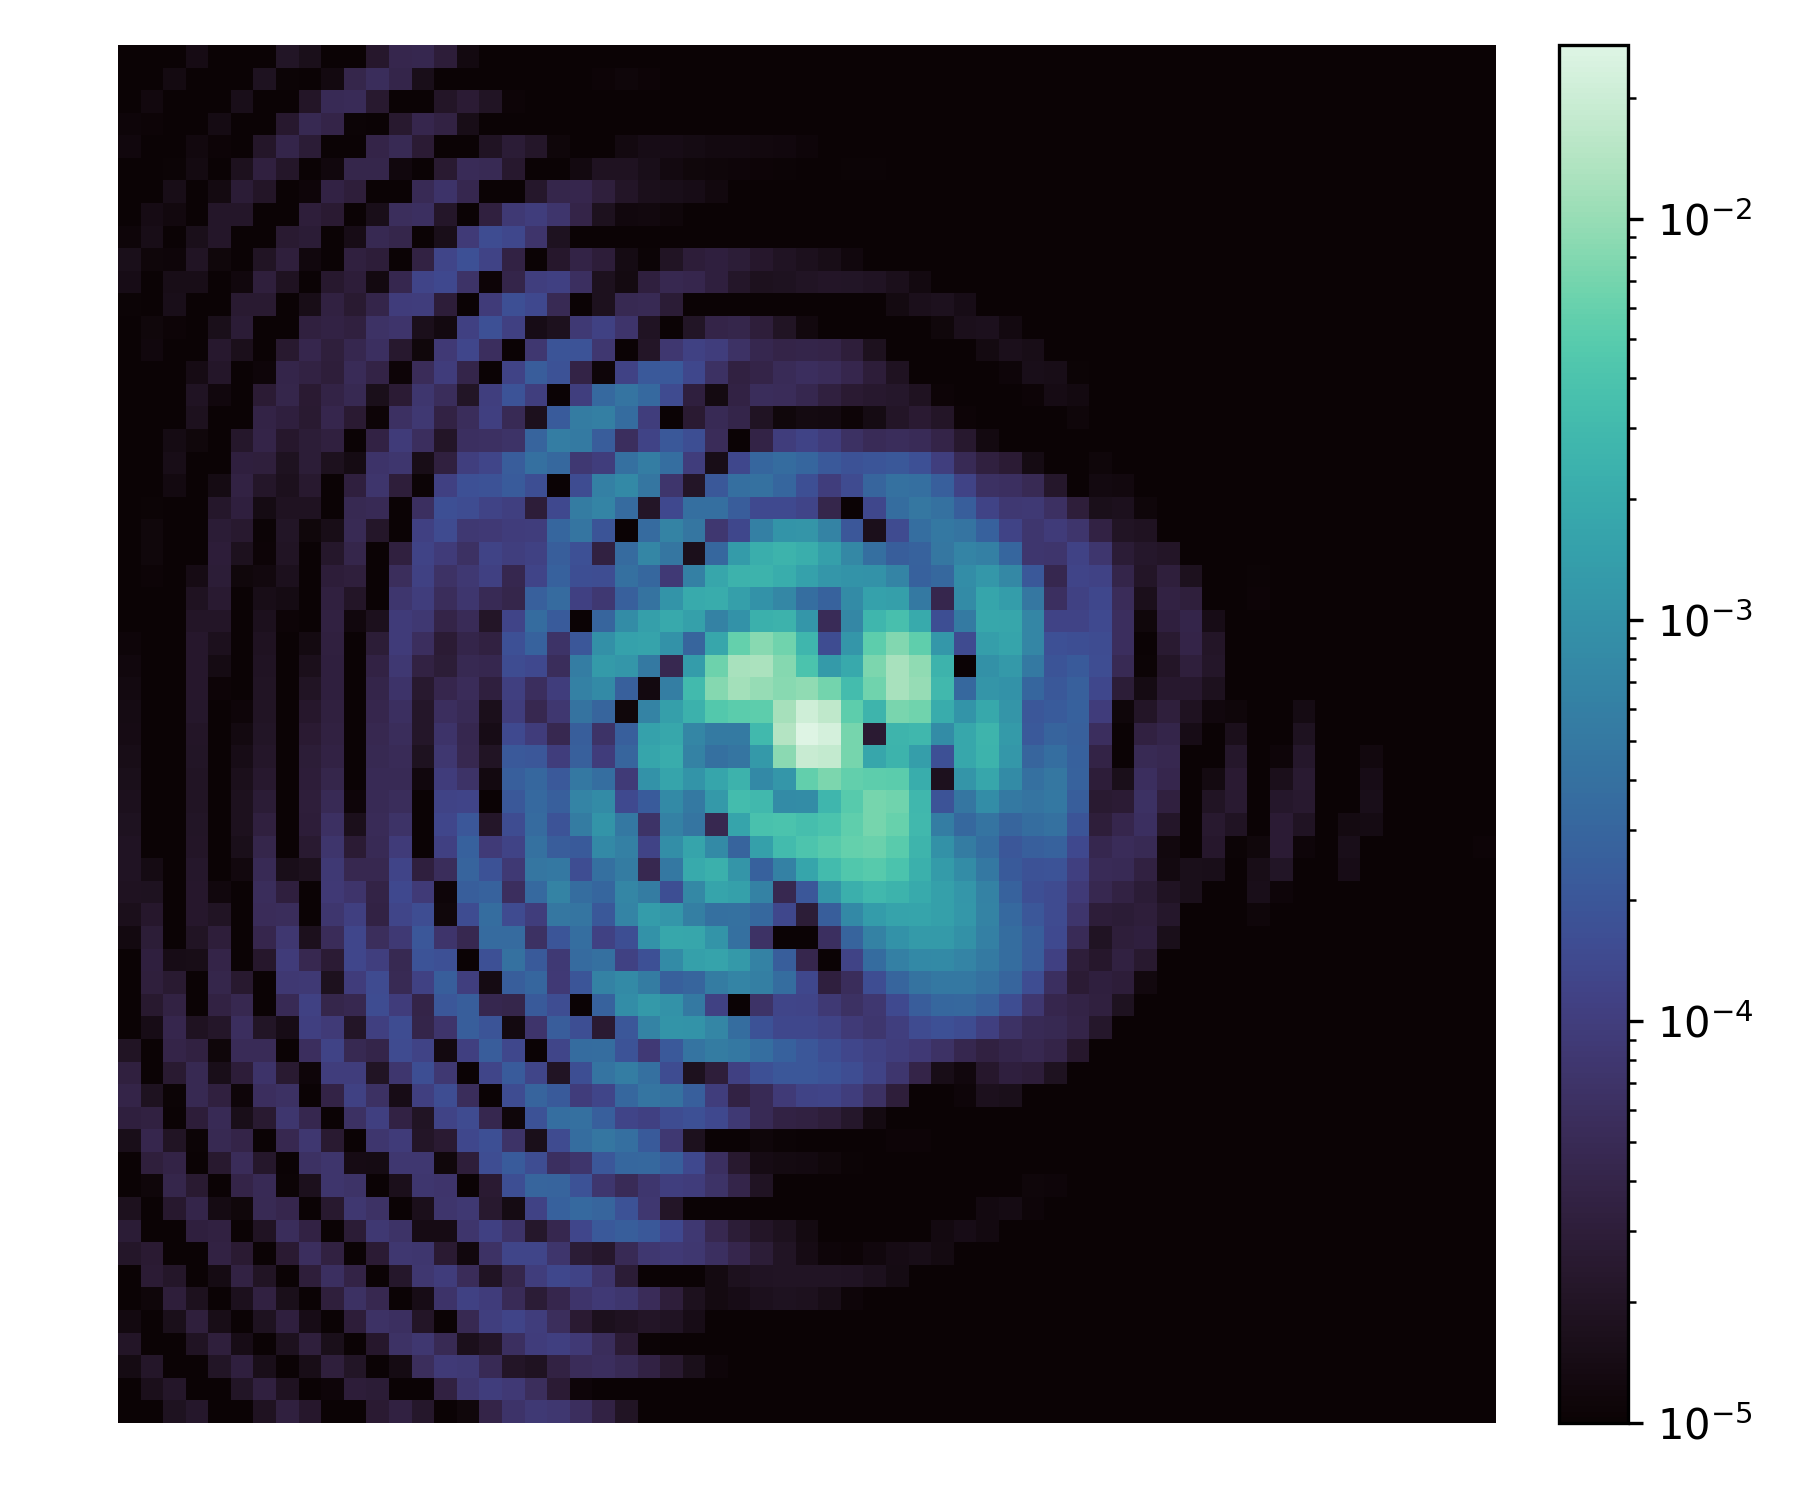
\includegraphics[width=0.7\textwidth]{img/exp4_4_psf.png}
    \caption{Esta imagen muestra la PSF del telescopio Sunrise. Se muestra en escala logaritmica para poder observar mejor la caída de la intensidad en los anillos de difracción.}
    \label{fig:psfReal}
\end{figure}


\subsubsection{Algoritmo de Richarson-Lucy}

Entonces, al igual que antes, cogemos una longitud de onda arbitraria y realizamos la deconvolución con el método de Richardson-Lucy. El resultado es el siguiente:

\begin{figure}[H]
    \centering
    \includegraphics[width=0.9\textwidth]{img/exp4_1_intensidad.png}
    \caption{Intensidad de la imagen deconvolucionada con el método de Richardson-Lucy. En la parte izquierda se muestra la imagen original, mientras que en la parte derecha se muestra la imagen deconvolucionada. Se puede observar que la imagen deconvolucionada tiene más detalle y contraste que la imagen original.}
    \label{fig:intensidadDecoReal}
\end{figure}

Visualmente ya se nota que Richardson-Lucy hace bien su trabajo. Rescata detalles de la imagen que antes estaban difuminados y le da un "empujón" importante al contraste general. 

El problema ahora a la hora de medir esta mejora es que estamos ante datos reales: no existe una "imagen ideal" con la que compararnos, así que las métricas SSIM y RMSE ya no nos sirven. Para sortear esto, tiramos de la métrica RMS (\textit{Contraste Cuadrático Medio}), que simplemente mide el contraste interno de la imagen:
\begin{equation}
    RMS = \sqrt{\frac{1}{N} \sum_{i=1}^{N} (I_i - \bar{I})^2}
\end{equation}

La lógica aquí es sencilla: a mayor RMS, más contraste y, en principio, más detalle fino habremos recuperado. En números, pasamos de un RMS inicial de $0.2028$ a $0.2193$ tras la deconvolución. Es una subida del $8.2\%$, lo que confirma numéricamente la mejora en contraste que ya apreciábamos a simple vista.

\subsubsection{Medición del campo magnético}
Ahora mediremos el algoritmo de Noor para medir el campo magnético a partir de la señal de Stokes $I$ y $V$. Para observar mejor los resultados, observaremos una región de interés de la imagen, que es la siguiente tras deconvolucionarlo con el algoritmo:

\begin{figure}[H]
    \centering
    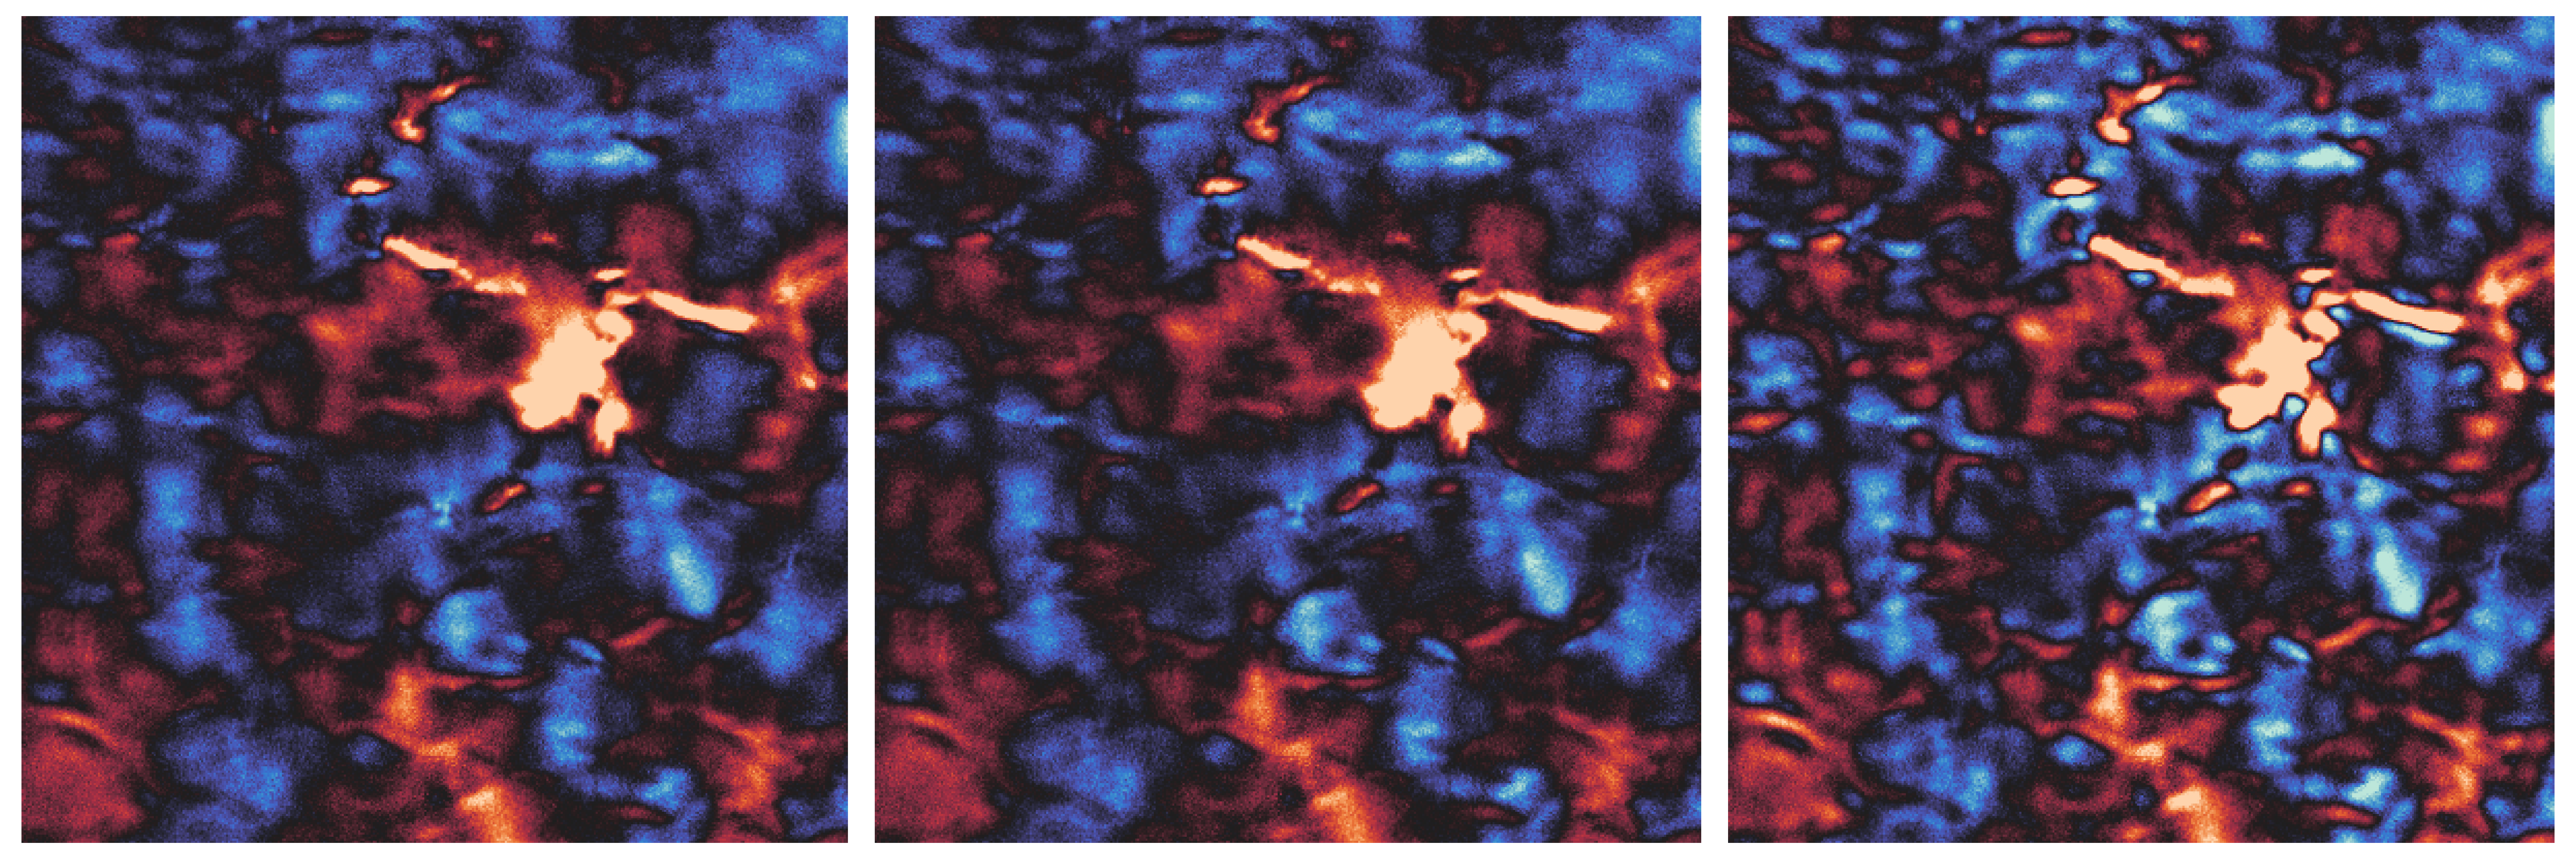
\includegraphics[width=0.9\textwidth]{img/exp4_3_campoB_zoom.png}
    \caption{Campo magnético medido a partir de la señal de Stokes $I$ y $V$ mediante el método adaptado de Noor. Se observa que el campo magnético tiene una estructura más definida y detallada que la imagen original.}
    \label{fig:campoMagDecoReal}
\end{figure}

Al igual que antes, se observa que el método logra recuperar la estructura del campo magnético, y se observan detalles que no se veían en la imagen original. Esto indica que el método es capaz de medir el campo magnético a partir de la señal de Stokes $I$ y $V$ de manera efectiva. 

Sin embargo, usar la métrica de RMS aquí no es muy buena idea, ya que el campo magnético tiene polaridades positivas y negativas que al sumarse podrían cancelarse y falsear el contraste. Para evitar este problema, usamos una métrica de nitidez basada en la \textit{varianza del Laplaciano}. Como el Laplaciano se encarga de aislar las altas frecuencias (donde viven los bordes y los detalles finos), su varianza nos da una medida muy fiable de cuánta estructura "nítida" hay en la imagen: $nitidez = Var(\nabla^2 B)$. 

Haciendo los números, la nitidez del campo magnético de partida es de $1.96 \times 10^2$, mientras que tras nuestro método sube a $2.03 \times 10^2$. Esta ganancia de un $3.6\%$ demuestra que, efectivamente, la técnica está logrando afinar los detalles de la estructura magnética del Sol con datos completamente reales.

Si vemos la imagen de diferencias entre la imagen original y la deconvolucionada, obtenemos el siguiente resultado:

\begin{figure}[H]
    \centering
    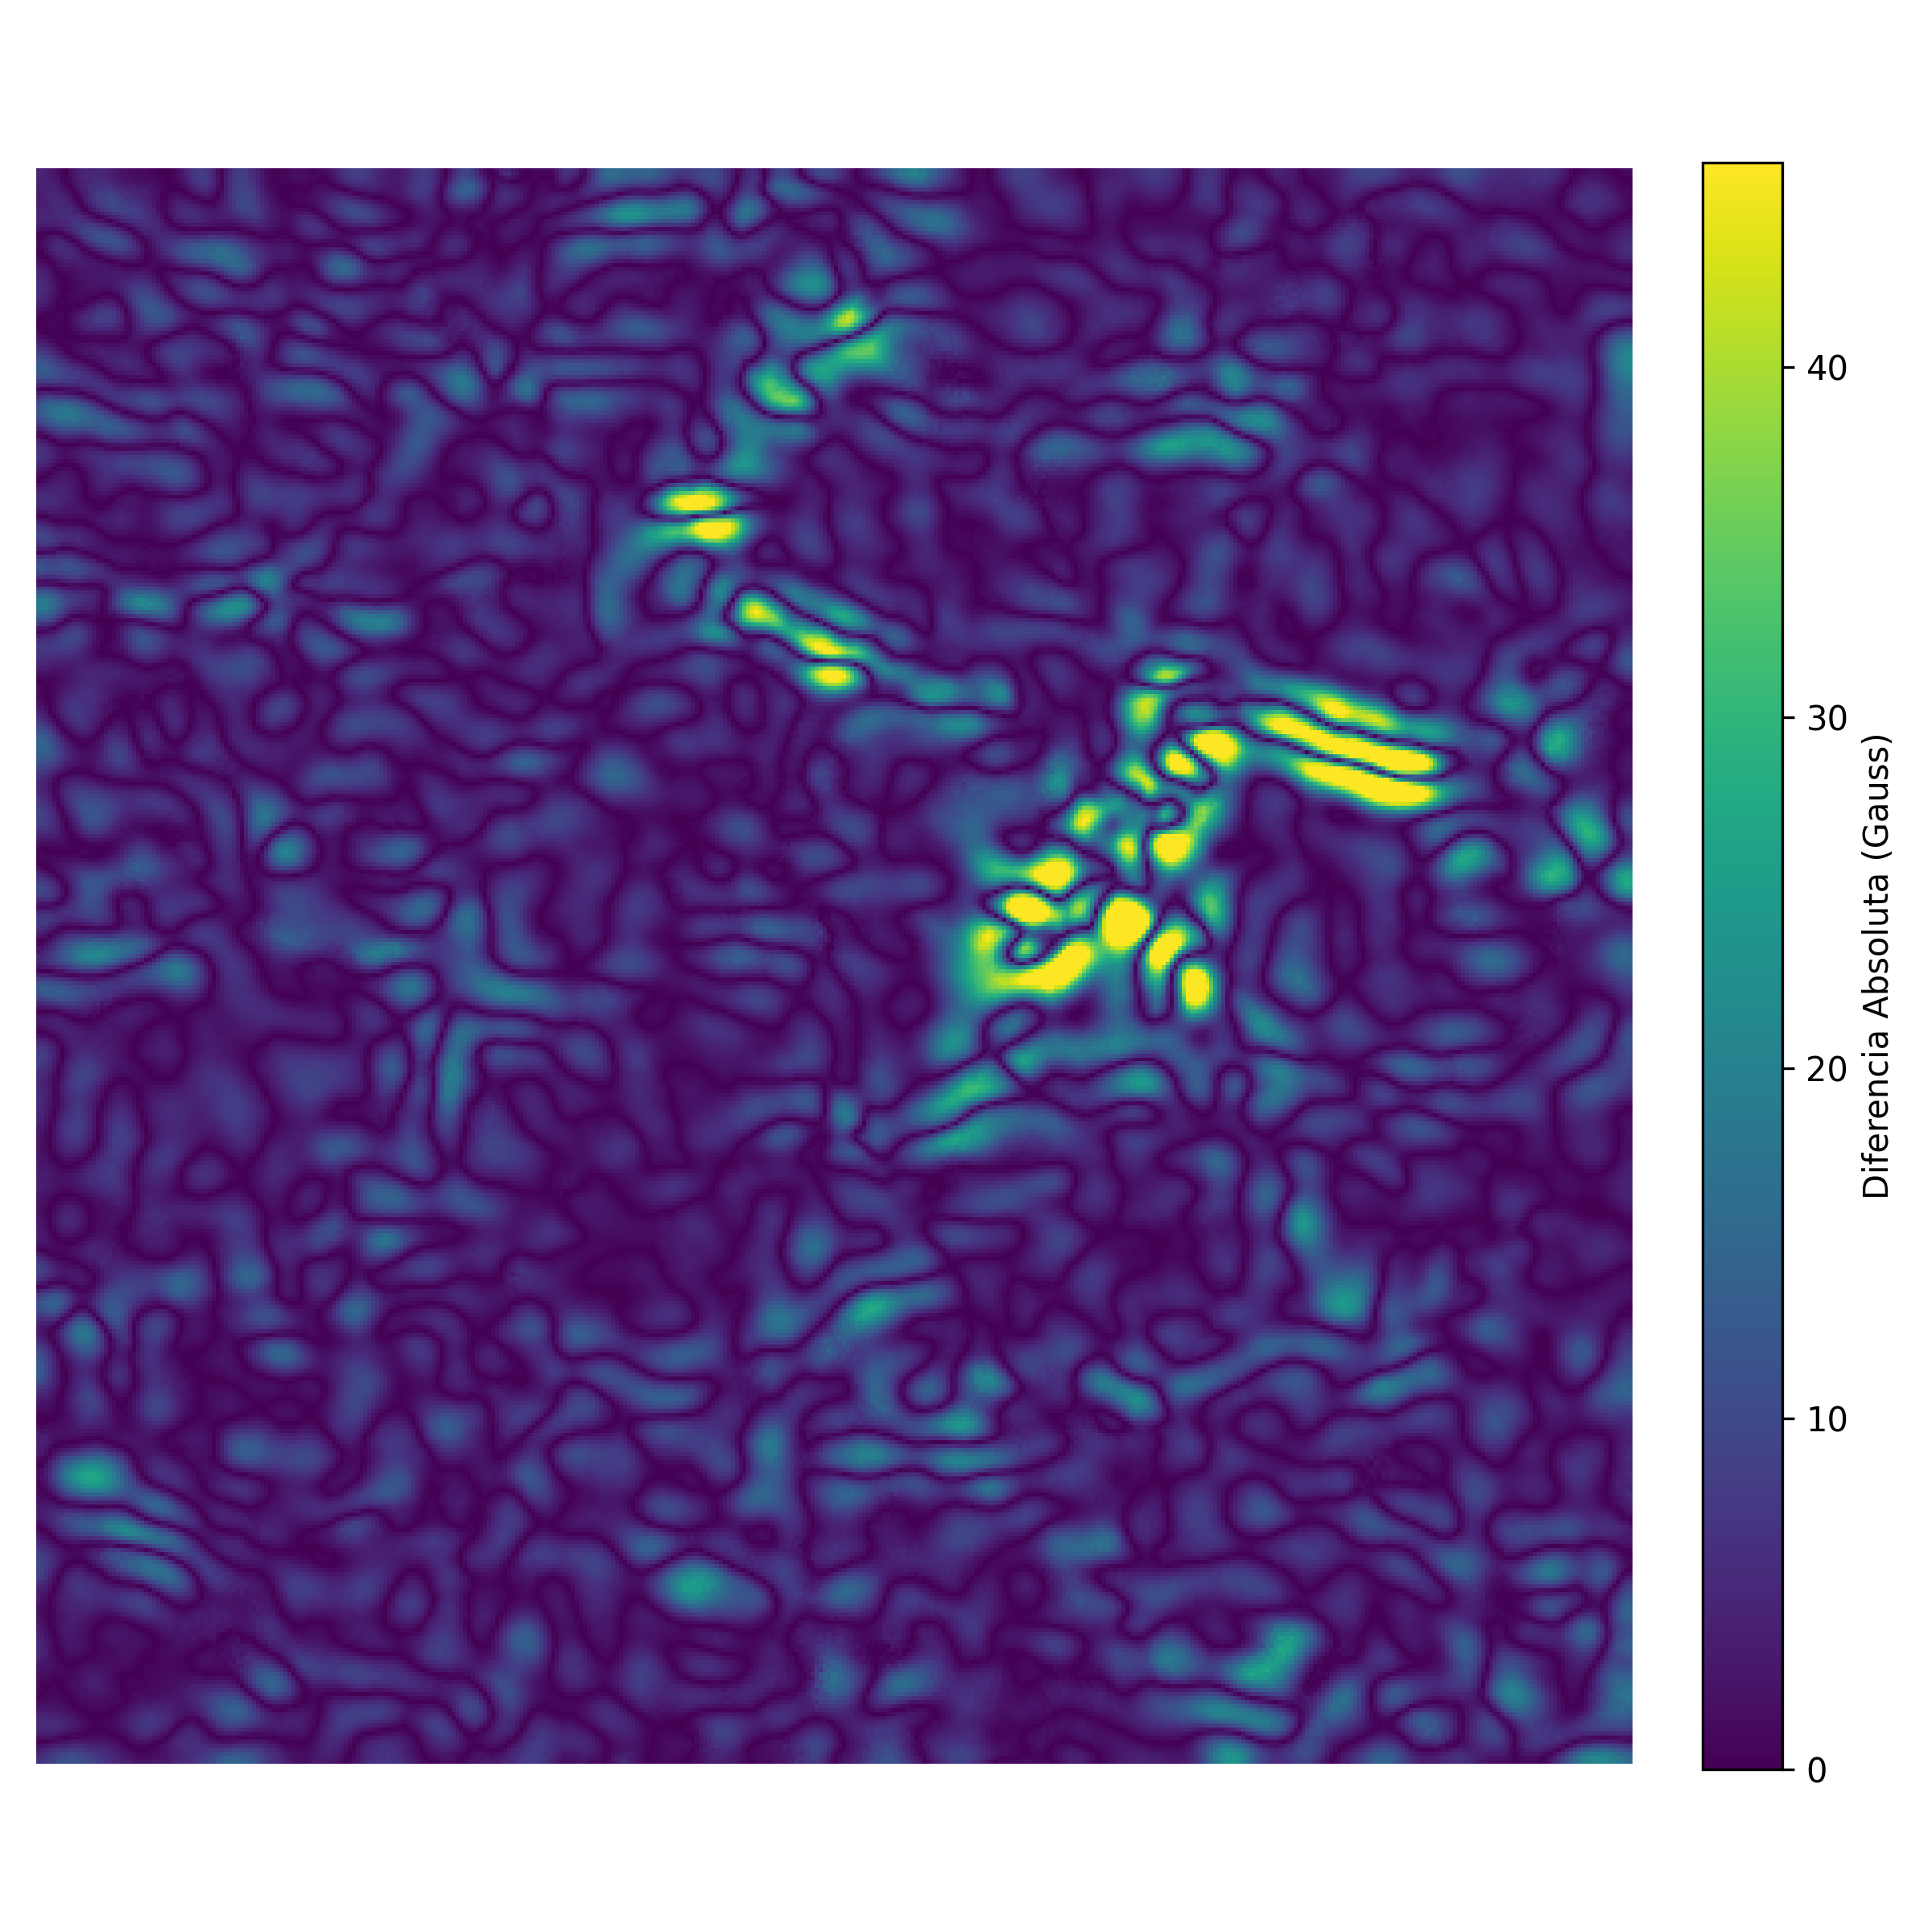
\includegraphics[width=0.9\textwidth]{img/exp4_5_diferencia.png}
    \caption{Mapa de diferencias entre la imagen original y la deconvolucionada del campo magnético, restando las imágenes. Se observa que las diferencias se concentran en las regiones donde el método logra recuperar detalles finos de la estructura del campo magnético.}
    \label{fig:campoMagDecoRealDiferencias}
\end{figure}

Se puede observar que las zonas más brillantes (colores verdes y amarillos) trazan los contornos y fronteras de la estructura magnética, indicando que el algoritmo está reconcentrando el flujo magnético en las zonas que fueron esparcidas por la PSF. 


\clearpage
% !TeX root = ../main.tex

\section{Conclusión}



\appendix
% !TeX root = ../main.tex


\section{Tecnologías usadas}
\label{sec:tecnologias_usadas}
Debido a la naturaleza computacional de este proyecto, el lenguaje principal de programación empleado ha sido \texttt{Python}, destacando por su legibilidad y amplia adopción en la comunidad astrofísica. Como base para la manipulación y vectorización de datos se utilizó \texttt{Numpy}, mientras que la librería \texttt{Astropy} facilitó el manejo de datos observacionales reales en formato \texttt{FITS}. 

Para el procesamiento de las imágenes, se empleó \texttt{Scipy}, cuyos módulos proporcionan herramientas esenciales como la convolución, transformadas de Fourier y algoritmos de optimización (aplicados en las secciones \ref{sec:metodosDeconvolucion} y \ref{sec:metodoDes}). Además, esta librería permitió paralelizar fácilmente el código.

Por último, se ha utilizado la inteligencia artificial como una potente herramienta de apoyo metodológico durante todo el proyecto, destacando en tres áreas principales:

\begin{itemize}
    \item Para facilitar y acelerar la comprensión de conceptos teóricos complejos abordados en la literatura científica.
    \item Para agilizar la localización de errores en el código y asistir en la generación de scripts para la visualización de datos y gráficas.
    \item Como soporte ortográfico y de corrección de estilo para mejorar la calidad en la redacción de este documento.
\end{itemize}

\clearpage

\addcontentsline{toc}{section}{Referencias} % Elige según idioma
%\addcontentsline{toc}{section}{References} % Elige según idioma

% Estilo de la bibliografía (aipnum4-2 para estilo American Institute of Physics)
\bibliographystyle{aipnum4-2} 
% Archivo exportado desde Zotero (sin poner la extensión .bib)
\bibliography{referencias,referencias_nuevas} 

\end{document}
